\documentclass[11pt,a4paper]{article}
\usepackage[utf8]{inputenc}
\usepackage[german]{babel}
\usepackage[T1]{fontenc}
\usepackage{amsmath}
\usepackage{amsfonts}
\usepackage{amssymb}
\usepackage{graphicx}
\usepackage[margin=1.25cm]{geometry} % Puts the same margin on all borders of the document

% Packages

\usepackage{hyperref} % Generate hyperlinks to referenced items
\usepackage{adjustbox} % Used to change parameters in \includegraphics[scale=•]{•}
\usepackage{enumitem} % Provides several options for lists
\usepackage{verbatim} % Package to use \begin{comment}
\usepackage{pdfpages} % Used to import PDF pages
\usepackage{multirow} % Allows us to have a single cell in a table span multiple rows
\usepackage{makecell} % Allows us to format multiple lines in a single cell
\usepackage{listings} % Used to type code in \begin{lstlisting}
\usepackage{xcolor}  % Gives access to coloring text
\usepackage{longtable} % Allows us to create a table over multiple pages
\usepackage{float} % Improved placement of floating items
\usepackage{pdfpages} % Used to import pdf pages
\usepackage{booktabs} % Used for horizontal lines instead of \hline



% Settings

\graphicspath{{./files/}} % Sets path for files to the files folder in the same directory

\hypersetup{
    colorlinks=false, %set true if you want colored links
    linktoc=all,     %set to all if you want both sections and subsections linked
    linkcolor=blue,  %choose some color if you want links to stand out
}


\begin{titlepage}
  \title{FOP Reference Sheet} % document_name-type_of_document
  \author{Frederick Wichert}
  \date{Last Edited: \today}
\end{titlepage}


\begin{document}
	\pagenumbering{gobble}
	\maketitle
	
	\setcounter{secnumdepth}{1}
	\setcounter{tocdepth}{1}
	\tableofcontents
	
	\newpage
	\pagenumbering{arabic}
		
\section{Definitionen}


	\begin{table}[H]
	\label{Definitionen}
	\begin{tabular}{ | p{4cm} p{13.5cm} | }	
		
	\hline
	\makecell[l]{Scope} & 
	\makecell[l]
	{
	$\rhd$ Sichtbarkeitsbereich von Definitionen und Identifiern \\
	\hspace{0.5cm} - Variablen müssen erst geschrieben werden, bevor sie 
	gelesen werden	
	} \\ \hline	
	
	\makecell[l]{Literale} & 
	\makecell[l]
	{
	$\rhd$ Literal (wörtlich) value einer Variable (5, "Hello", true, 
	null, etc.) 
	} \\ \hline
	
	\makecell[l]{Identifier} & 
	\makecell[l]
	{
	$\rhd$ Identifizieren Entitäten, alles selbsbenannte (Klassen, 
	Variablen)
	} \\ \hline
	
	\makecell[l]{Konversion (Casting)} & 
	\makecell[l]
	{
	$\rhd$ Schreibt man einen Typen in Klammern vor einen Wert oder 
	eine Variabel, \\ 
	\hspace{0.5cm} ((int) new short(5)) wird der Typ konvertiert
	} \\ \hline
	
	\makecell[l]{Ternärer Operator} & 
	\makecell[l]
	{
	$\rhd$ BoolescherAusdruck ? IfValue : ElseValue
	} \\ \hline

	\makecell[l]{rvalue u. lvalue} & 
	\makecell[l]
	{
	$\rhd$ Rechtsaudrücke (rvalue) haben Typ und Wert \\
	\hspace{0.4cm} - z.B. Zuweisungen, Initialisierungen etc. \\
	$\rhd$ Linksausdrücke (lvalue) verweisen auf Speicherstelle \\
	\hspace{0.4cm} - z.B. Linke seite einer Zuweisung	
	} \\ \hline	

	\makecell[l]{Zuweisungen} & 
	\makecell[l]
	{
	$\rhd$ Werden von rechts nach links abgearbeitet \\
	\hspace{0.4cm} - z.B. \texttt{a = b += d *= f;} \\
	$\rhd$ Durch das Semikolon wird aus dem Ausdruck eine Anweisung \\
	$\rhd$ Zuweisungen haben Seiteneffekt \\
	$\rhd$ \texttt{var1 operator= var2} ist gleich \texttt{var1 = var1 operator var2} \\
	\hspace{0.4cm} - z.B. \texttt{a *= b;} ist gleich \texttt{a = a * b;}
	} \\ \hline

	\makecell[l]{Switch} &
	\makecell[l]
	{
	$\rhd$ Unterscheideds zwischen möglichen werten einer Variable \\
	\hspace{0.4cm} \texttt{switch (number) \{} \\
	\hspace{0.4cm} \texttt{		case 3:} \\
	\hspace{0.4cm} \texttt{		\hspace{0.1cm} System.out.println("It is prime");} \\
	\hspace{0.4cm} \texttt{		\hspace{0.1cm} break;} \\
	\hspace{0.4cm} \texttt{		case 5:} \\
	\hspace{0.4cm} \texttt{		\hspace{0.1cm} System.out.println("It is prime as well");} \\
	\hspace{0.4cm} \texttt{		\hspace{0.1cm} break;} \\
	\hspace{0.4cm} \texttt{		default:} \\
	\hspace{0.4cm} \texttt{		\hspace{0.1cm} System.out.println("This happens when neither case is true");} \\
	\hspace{0.4cm} \texttt{\}} \\
	$\rhd$ Hinter case muss immer ein Literal stehen, und keine Variable \\
	$\rhd$ Um Endlosschleifen zu vermeiden ist es sinnvoll \texttt{default:} zu implementieren \\
	$\rhd$ Jeder case sollte mit einem break; beendet werden \\
	} \\ \hline
	
	
	\end{tabular}
	\end{table}
	
	
	
	\begin{figure}[H]
		\centering
		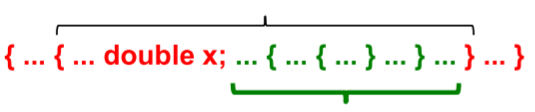
\includegraphics[scale=0.7]{scope_variable}
		\caption{Scope von Variablen}
	\end{figure}


	
\newpage



\section{Computerspeicher}


	\begin{table}[H]
	\label{Computerspeicher}
	\begin{tabular}{ | p{4cm} p{13.5cm} | }
	
	
	\hline		
	\makecell[l]{Unsere Vorstellung} & 
	\makecell[l]
	{
	$\rhd$ gro\ss es Feld aus Maschinenwörtern mit eindeutiger Adresse
	} 	\\ \hline
	
	\makecell[l]{Primitve Datentypen} & 
	\makecell[l]
	{
	$\rhd$ Name verwei\ss t tatsächelich auf auf die Speicherstelle
	} 	\\ \hline
	
	\makecell[l]{Objekte im \\ 
				 Computerspeicher} & 
	\makecell[l]
	{
	$\rhd$ 
	Beim erzeugen wird ausreichend gro\ss er Speicherplatz reserviert
	} 	\\ \hline
	
	\makecell[l]{Attribute} & 
	\makecell[l]
	{
	$\rhd$ Werden relativ zur Anfangsadresse des Objektes gespeichert
	} 	\\ \hline
	
	\makecell[l]{Programm zu Prozess} & 
	\makecell[l]
	{
	$\rhd$ (Java-) Quellcode zu (Java-) Bytecode, dieser wird 
	ausgeführt \\
	$\rhd$ Das Ausführen nennt man Prozess \\
	$\rhd$ Mehrere Prozesse laufen parallel \\
	$\rhd$ Durch teilen der Prozessorkern Zeit laufen Prozesse quasi 
	parallel
	} 	\\ \hline
	
	\makecell[l]{Abarbeitung der \\ 
	Anweisungen} & 
	\makecell[l]
	{
	$\rhd$ Programm Counter, speziell resveriert, enthält 
	Speicheradresse der \\ 
	nächsten Anweisung \\
	$\rhd$ Wird nach Ausführung erhöht, und verweist auf nächst 
	Anweisung \\
	$\rhd$ Bei Sprunganweisungen (Schleifen) wird er einfach 
	überschrieben
	} 	\\ \hline	
	
	\makecell[l]{Garbage Collector} & 
	\makecell[l]
	{
	$\rhd$ Der Garbage Collector ist teil des Laufzeitsystems \\
	$\rhd$ Wird hin und wieder aufgerufen werden, kann aber optimiert werden \\
	$\rhd$ Gibt alle nicht erreichbaren Speicherplatz frei
	} 	\\ \hline

	
	\end{tabular}
	\end{table}
	

	\begin{center}
	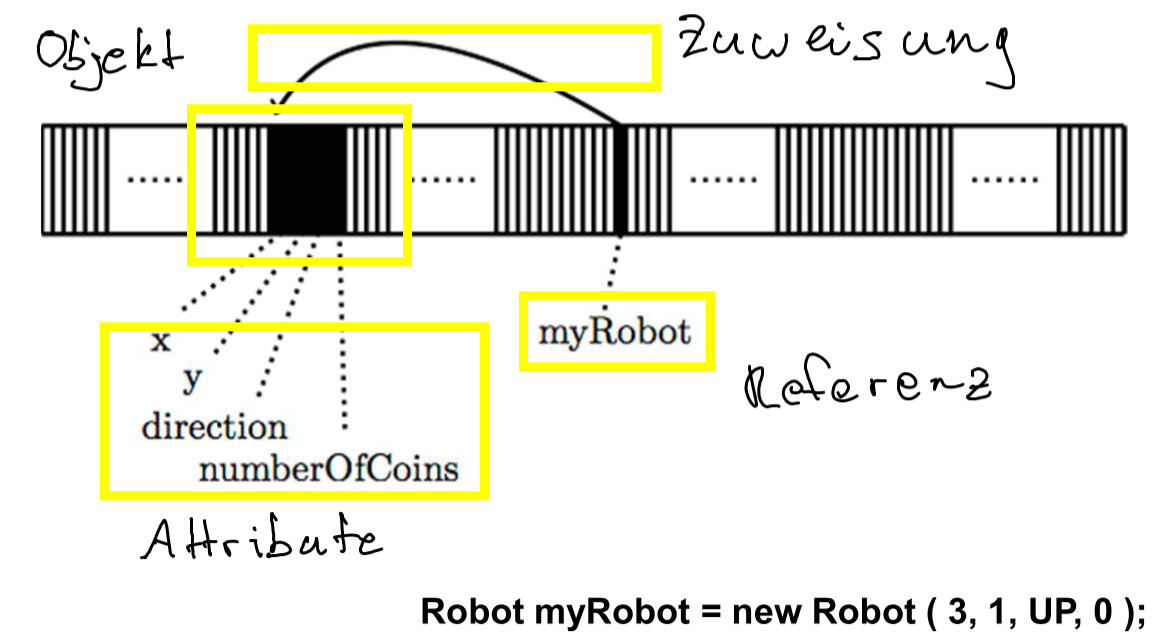
\includegraphics[scale=0.5]{computerspeicher}
	\end{center}
	
	
	
\section{Datenstrukturen}


	\begin{table}[H]
	\label{Datenstrukturen}
	\begin{tabular}{ | p{4cm} p{13.5cm} | }
	
	
	\hline	
	\makecell[l]{Zugriff} &
	\makecell[l]
	{
	$\rhd$ Verschiedene Arten, z.B.: \texttt{int myNumber;} \\
	\hspace{0.5cm} - Schreibend: \texttt{myNumber = 5;} \\
	\hspace{0.5cm} - Lesend: \texttt{otherNumber = myNumber;} \\
	$\rhd$ Referenz muss erst beschrieben werden um gelesen zu werden \\
	}	\\ \hline
	
	\makecell[l]{Arrrays} & 
	\makecell[l]
	{
	$\rhd$ Zum speichern Variablen selben Types \\
	$\rhd$ Statische grö\ss e, nicht mehr veränderbar \\
	$\rhd$ Typ[] array = new Typ[n]; \\
	$\rhd$ n gibt die Menge der Variablen an \\
	$\rhd$ kann von Objekten wie von primitiven Datentypen erzuegt 
	werden
	} 	\\ \hline
	
	\makecell[l]{X} & 
	\makecell[l]
	{
	$\rhd$ X
	} 	\\ \hline

	
	\end{tabular}
	\end{table}
	


\section{Klassen und Objekte}

\subsection{Klassen}
	\begin{table}[H]
	\label{Klassen}
	\begin{tabular}{ | p{4cm} p{13.5cm} | }


	\hline
	\makecell[l]{Attribute} & 
	\makecell[l]
	{
	$\rhd$ Eigenschaften einer Klasse, bzw. des Objektes \\
	$\rhd$ z.B. privat int weight; \\
	$\rhd$ z.B. public String name; \\
	$\rhd$ \texttt{static} Deklarierte Attribute hei\ss en Klassenattribute \\
	\hspace{0.4cm} - Bei Objekterzeugung wird nicht immer eine Kopie erzeugt \\
	\hspace{0.4cm} - Nur eine einzige Speicherstelle für die ganze Klasse \\
	$\rhd$ Zugriff über \texttt{myObject.attribute} oder über \texttt{MyClass.attribute} \\
	} 	\\ \hline

	\makecell[l]{Sichtbarkeit} & 
	\makecell[l]
	{
	$\rhd$ Entweder \texttt{public} oder gar nichts \\
	$\rhd$ Nur eine public Klasse oder Interface pro Datei \\
	$\rhd$ Diese muss den Namen der Datei haben \\
	$\rhd$ Nicht public entspricht \texttt{private}
	} 	\\ \hline
	
	\makecell[l]{Kontruktor} & 
	\makecell[l]
	{
	$\rhd$ Selber Name wie die Klasse, kein Rückgabewert \\
	$\rhd$ Hat \textbf{keinen} Rückgabewert, z.B. \texttt{public 
	MyClass \{ ... \}} \\
	$\rhd$ Falls kein Konstruktor definiert ist, wird Standardkonstruktor genutzt \\
	$\rhd$ kann natürlich auch überladen werden
	} 	\\ \hline
	
	\makecell[l]{Abtraktion} & 
	\makecell[l]
	{
	$\rhd$ Klasse kann abstrakt sein, muss es aber sobald eine 
	Methode abstrakt ist \\
	$\rhd$ Hat Klasse eine abstrakte Methode muss sie auch abstrakt 
	definiert sein \\
	$\rhd$ z.B. \texttt{abstract public MyClass} \\
	$\rhd$ Keine Objekterzeugung möglich \\
	$\rhd$ Siehe \underline{\nameref{Methoden}} \\
	$\rhd$ Bei Vererbung müssen \textbf{nicht} alle abstrakten Methoden 
	implementiert werden \\
	$\rhd$ Siehe \underline{\nameref{Vererbung}}
	} 	\\ \hline

	\makecell[l]{java.lang.Object} & 
	\makecell[l]
	{
	$\rhd$ Erbt eine Klasse nicht, so erbt sie von \texttt{java.lang.Object} \\
	$\rhd$ \texttt{lang.Object} hat diverse Klassenmethoden \\
	\hspace{0.4cm} - z.B. \texttt{public boolean equals (Object obj) \{...\}} \\
	\hspace{0.4cm} - z.B. \texttt{public String toString () \{...\}} \\
	} 	\\ \hline

	\makecell[l]{static initializer} & 
	\makecell[l]
	{
	$\rhd$ Die besondere Static Methode: Kopf besteht nur aus dem Wort static \\
	\hspace{0.4cm} - \texttt{static \{ ... \}} \\
	$\rhd$ Wird zu Beginn der Abarbeitung des Programms ausgeführt \\
	$\rhd$ z.B. zur Initialisierung von Konstanten etc.
	} 	\\ \hline
		
	
	\end{tabular}
	\end{table}
	
\subsection{Objekte}
	\begin{table}[H]
	\label{Objekte}
	\begin{tabular}{ | p{4cm} p{13.5cm} | }
	
	
	\hline
	\makecell[l]{Erzeugung} & 
	\makecell[l]
	{
	$\rhd$ Kann nur von \underline{\nameref{Klassen}} erzeugt werden \\
	$\rhd$ Beim erstellen wird der Konstruktor (Siehe: 
	\underline{\nameref{Klassen}} mittels "\texttt{new}" aufgerufen \\
	$\rhd$ z.B. \texttt{MyClass myObject = new MyClass();}
	} 	\\ \hline
	
	\makecell[l]{Kopieren} & 
	\makecell[l]
	{
	$\rhd$ Shallow vs Depp Copy \\
	\hspace{0.5cm} - Shallow: Kopieren der Referenzadresse \\
	\hspace{0.5cm} - Deep: Kopieren der Werte in ein neues Objekt \\
	$\rhd$ Beim erstellen wird der Konstruktor (Siehe: 
	\underline{\nameref{Klassen}} mittels "\texttt{new}" aufgerufen \\
	$\rhd$ z.B. \texttt{MyClass myObject = new MyClass();}
	} 	\\ \hline
	
	
	\end{tabular}
	\end{table}
	
	

\section{Referenzen}


	\begin{table}[H]
	\label{Referenzen}
	\begin{tabular}{ | p{4cm} p{13.5cm} | }
	
	
	\hline
	\makecell[l]{Funktion} & 
	\makecell[l]
	{
	$\rhd$ Verweist mittels einer Speicheraddresse auf den Stack \\
	$\rhd$ Verwendet bei Objekten etc. Nicht bei primitven Datentypen \\
	$\rhd$ Vergleich (Gleicheit: \texttt{==}) nur \texttt{true} bei 
	gleicher Referenz, trotz "Wertgleichheit"
	} 	\\ \hline
	
	\makecell[l]{Verwendung} & 
	\makecell[l]
	{
	$\rhd$ Referenztypen können quasi alles au\ss er primitven Datentypen 
	sein \\
	$\rhd$ D.h. Klassen, Interfaces und Enumerationen \\
	$\rhd$ z.B. \texttt{MyClassIntfEnum reference = ... ; } \\
	$\rhd$ "Gefä\ss e" um direkt oder indirekt abgeleitete Entitäten zu 
	speichern \\
	$\rhd$ Wo der Referenztyp steht, können Subtypen verwendet werden
	} 	\\ \hline
	
	\makecell[l]{Statisch vs. Dynamisch} & 
	\makecell[l]
	{
	$\rhd$ z.B. \texttt{MyStaticTyppe sample = MyDynamicType();} \\
	$\rhd$ Zugriff nur auf Funktionen und Werte die in beiden Typen 
	definiert sind, \\
	\hspace{0.4cm} also nicht auf eine Funktion die nur in 
	\texttt{MyDynamicType} 	zu finden ist, \\
	\hspace{0.4cm} umgekehrt ist dies gar nicht möglich
	} 	\\ \hline
	
	
	\end{tabular}
	\end{table}



\section{Enumerationen}


	\begin{table}[H]
	\label{Enumerationen}
	\begin{tabular}{ | p{4cm} p{13.5cm} | }


	\hline
	\makecell[l]{Funktion} & 
	\makecell[l]
	{
	$\rhd$ Wird von \texttt{java.lang.Enum} abgeleitet \\
	$\rhd$ Kann benutzt werden um Spezielle Wertbezeichner zu 
	erstellen \\
	$\rhd$ z.B. \texttt{public enum MyEnum \{UP, DOWN, LEFT, RIGHT\}} 
	\\
	$\rhd$ Davon können Variablen mit entsprechendem Wert erstellt 
	werden \\
	$\rhd$ Um nicht immer MyEnum.VALUE zu schreiben, \texttt{import 
	static MyEnum}
	} 	\\ \hline


	\makecell[l]{Klassenmethoden} & 
	\makecell[l]
	{
	$\rhd$ \texttt{MyEnumReference.vlaues()} \\
	\hspace{0.4cm} - liefert ein Array mit allen MyEnum Komponenten zurück \\ 
	\hspace{0.66cm} in Definitionsreihenfolge \\
	$\rhd$ \texttt{MyEnumReference.name)()} \\
	\hspace{0.4cm} - liefert den Namen des Objektes zurück \\
	} 	\\ \hline

	
	\end{tabular}
	\end{table}
	
	

\section{Methoden}


	\begin{table}[H]
	\label{Methoden}
	\begin{tabular}{ | p{4cm} p{13.5cm} | }
	

	\hline
	\makecell[l]{Aufbau} &
	\makecell[l]
	{
	$\rhd$ Bestehend aus Kopf (Head) und Rumpf (Body) \\
	$\rhd$ \texttt{public staic void main (String[]args) throws Exception} \\
	\hspace{0.4cm} - bestehend aus dem Namen, einem Identifier (nur eine 'main' Methode) \\
	\hspace{0.4cm} - dem Rückgabetyp, optional auch void \\
	\hspace{0.4cm} - den Modifiern, public, static, private etc. (Verändern 'nur' die Nutzung) \\
	\hspace{0.4cm} - der Paramterliste, spezifiert durch den Typen gefolgt vom Namen\\
	\hspace{0.4cm} - und die optionalen throws deklaration (Exception) \\
	$\rhd$ Die Signatur muss bei jeder Methode unterschiedlich sein
	} 	\\ \hline
	
	
	\makecell[l]{Ausfürung} & 
	\makecell[l]
	{
	$\rhd$ Stackpointer verweist auf die nächste Anweisung \\
	$\rhd$ Bei Aufruf einer Methode, Frame auf dem Callstack wird 
	erzeugt\\
	$\rhd$ Dieser bietet allen eventuell benötigten Speicherplatz 
	bereit \\
	$\rhd$ Sowie Verweis auf den Methoden beginn, und 
	Rücksprungadresse \\
	$\rhd$ Der Stackpinter verweist nun auf den Frame \\
	$\rhd$ Nach Ausführung wird Stackpointer auf 
	Rücksprungadresse gesetzt \\
	} 	\\ \hline
	
	
	\makecell[l]{Overloading} & 
	\makecell[l]
	{
	$\rhd$ Methoden gleichen Namens, unterschiedlicher Parameterliste
	werden differenziert \\
	$\rhd$ Siehe \underline{\nameref{Vererbung}}
	} 	\\ \hline
	
	
	\makecell[l]{Abtraktion} & 
	\makecell[l]
	{
	$\rhd$ Eine Methode kann abstrakt definiert sein \\
	$\rhd$ Diese hat keinen Methodenrumpf \\
	$\rhd$ z.B. \texttt{abstract public void myMethod} \\
	$\rhd$ Siehe \underline{\nameref{Klassen}}
	} 	\\ \hline


	\makecell[l]{Formal vs \\ Aktualparamter} & 
	\makecell[l]
	{
	$\rhd$ Die in dem Methodenkopf deklarierten Paramter nennt man Formalparamter \\
	$\rhd$ Diese entsprechen quasi lokalen Variablen in der Funktion \\
	$\rhd$ z.B. \texttt{public int sumFunction (int a, int b) \{...\}} \\
	$\rhd$ a, b sind in diesem Fall Formalparamter \\
	$\rhd$ Beim Aufruf werden sie durch Aktualparamter ersetzt \\
	$\rhd$ z.B. \texttt{sumFunction(13, 37)} \\
	} 	\\ \hline


	\hline
	\makecell[l]{Klassenmethoden} & 
	\makecell[l]
	{
	$\rhd$ Mit \texttt{static} deklarierte Methoden hei\ss en Klassenmethoden \\
	$\rhd$ Klassenmethoden \textbf{dürfen nicht}: \\
	\hspace{0.4cm} - Objektattribute lesen oder schreiben \\
	\hspace{0.4cm} - Objektmethoden aufrufen \\
	$\rhd$ Klassenmthoden \textbf{dürfen}: \\
	\hspace{0.4cm} - Klassenattribute lesen oder schreiben \\
	\hspace{0.4cm} - Klassenmethoden aufrufen \\
	$\rhd$ Können ohne Objektinitialisierung aufgerufen werden \\
	} 	\\ \hline

	
	\makecell[l]{Variable \\ Parameteranzahl} & 
	\makecell[l]
	{
	$\rhd$ Wird durch drei Punkte nach dem Variablentyp deklariert \\
	$\rhd$ z.B. \texttt{public static void m (char c, double... args)} \\
	\hspace{0.4cm} \texttt{\{ for (double x : args) \{ . code . \} \}} \\
	$\rhd$ Aufruf kann auf verschieden Arten erfolgen \\
	\hspace{0.4cm} - \texttt{X.m('c', new Array[])} \\
	\hspace{0.4cm} - \texttt{X.m('a', 23.1, 321, 57.3)} \\
	\hspace{0.4cm} - \texttt{X.m('b', 1337)} \\
	} 	\\ \hline


	\makecell[l]{Signatur} & 
	\makecell[l]
	{
	$\rhd$ Die Signatur einer Methode besteht aus Name, und Parameterliste
	} 	\\ \hline

	
	\end{tabular}
	\end{table}
	
	
	\begin{figure}[H]
		\centering
		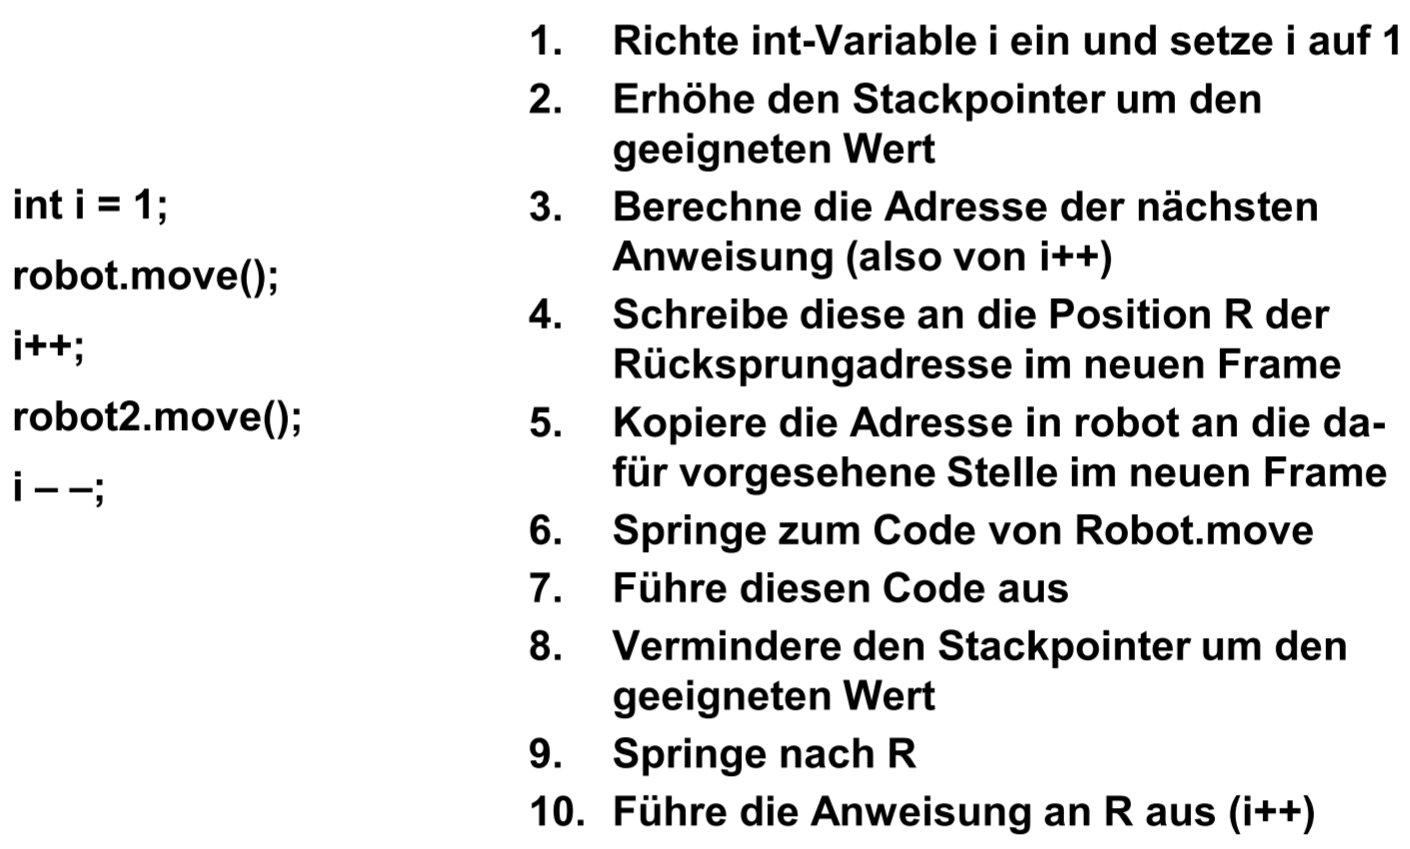
\includegraphics[scale=0.4]{methodenaufruf}
		\caption{FoP-Bot Methodenaufruf}
	\end{figure}
	


\section{Interfaces}


	\begin{table}[H]
	\label{Interfaces}
	\begin{tabular}{ | p{4cm} p{13.5cm} | }


	\hline
	\makecell[l]{Struktur} & 
	\makecell[l]
	{
	$\rhd$ Sind ähnlich aufgebaut wie \underline{\nameref{Klassen}} 
	aber komplett abstrakt \\
	$\rhd$ Implementierung wie folgt: \texttt{public MyClass implements 
	MyInterface} \\
	$\rhd$ Abstrakte Methoden werden nicht implementiert sondern nur 
	definiert \\
	$\rhd$ Alle Methoden müssen \texttt{public} sein \\
	} 	\\ \hline
	
	\makecell[l]{Funktion} & 
	\makecell[l]
	{
	$\rhd$ z.B. \texttt{public MyClass implements MyInterface, Interface2} 
	\\
	$\rhd$ Alle Methoden müssen in \texttt{MyClass} implementiert 
	werden \\
	$\rhd$ Dient der Modularität und der Fehlervermeidung \\
	$\rhd$ Wird bei Implementierung eine Methode nicht implementiert, ist 
	diese, \\
	\hspace{0.5cm} und somit die ganze Klasse abstrakt \\
	$\rhd$ Eine Klasse kann mehrer Interfaces implementieren
	} 	\\ \hline

	
	\end{tabular}
	\end{table}
	


\section{Vererbung}


	\begin{table}[H]
	\label{Vererbung}
	\begin{tabular}{ | p{4cm} p{13.5cm} | }


	\hline
	\makecell[l]{Funktion} & 
	\makecell[l]
	{
	$\rhd$ Reicht alle Methode und Funktionen weiter \\
	$\rhd$ z.B. \texttt{public class MyHeritageClass extends MyClass} \\
	$\rhd$ Eine Klasse kann maximal von einer anderen Klasse erben \\
	\hspace{0.5cm} - also keine Mehrfachvererbung (Ausnahme Interfaces) \\
	$\rhd$ Wo ein Referenztyp (Supertyp) erwartet wird kann ein 
	Subtyp genutzt werden \\
	\hspace{0.5cm} - aka. direkt oder indirekt abgeleitete Entitäten \\
	$\rhd$ Exceptionklasse durch abgeleitete Exceptionklasse ersetzbar \\
	} 	\\ \hline

	\makecell[l]{Suberkonstruktor} & 
	\makecell[l]
	{
	$\rhd$ Mit \texttt{super(x, y)} wird der Konstruktor der 
	Superklasse gerufen \\
	$\rhd$ Muss im Konstruktor vor allen anderen Anweisungen stehen \\
	$\rhd$ Siehe \underline{\nameref{Klassen}}
	} 	\\ \hline
	
	\makecell[l]{Overloading} & 
	\makecell[l]
	{
	$\rhd$ Vererbte Methoden können mit \textbf{anderer} Parameterliste 
	überschrieben werden \\
	$\rhd$ Siehe \underline{\nameref{Methoden}}
	} 	\\ \hline
	
	\makecell[l]{Overwrite} & 
	\makecell[l]
	{
	$\rhd$ Vererbte Methoden können mit \textbf{gleicher} Paramterliste 
	überschrieben werden \\
	$\rhd$ Dies bedeutet die Signatur muss gleich bleiben \\
	} 	\\ \hline
	
	\makecell[l]{Interfaces} & 
	\makecell[l]
	{
	$\rhd$ z.B. \texttt{public interface MyIntf extends Intf2, Intf3} \\
	\hspace{0.5cm} - Beispiel von "Mehrfachvererbung"
	} 	\\ \hline
	
	\end{tabular}
	\end{table}
	


\section{Zugriffsrechte und Packages}


	\begin{table}[H]
	\label{Zugriffsrechte und Packages}
	\begin{tabular}{ | p{4cm} p{13.5cm} | }


	\hline
	\makecell[l]{Packages} & 
	\makecell[l]
	{
	$\rhd$ Ist eine Zusammenfassung von Klassen, Interfaces und/oder 
	Enumerationen \\
	\hspace{0.5cm} - Normale Verzeichnisstruktur \\
	\hspace{0.5cm} - In Subpackages unterteilst \\
	$\rhd$ Dient unter anderem der Vermeidung von Namenskonflikten \\
	$\rhd$ Deklariert mit \texttt{package mypackage} \\
	$\rhd$ Importiert mit \texttt{import package.subpackage.class} \\
	\hspace{0.5cm} oder mit \texttt{import package.subpackage.*;} \\
	\hspace{0.5cm} um alle Klassen in \texttt{subpackage} zu importieren\\
	\hspace{0.5cm} weitere Subpackages werden nicht importiert \\
	$\rhd$ \texttt{java.lang.*} wird automatisch vom Compiler importiert
	} 	\\ \hline

	\makecell[l]{Zugriffsrechte} & 
	\makecell[l]
	{
	$\rhd$ \texttt{private}, Nur in der Klasse selbst \\
	$\rhd$ \texttt{keine Angabe}, Zusätzlich zu (Package) Private - im 
	ganzen Package 
	sichtbar \\
	$\rhd$ \texttt{protected}, Zus. zu keine Angabe - in allen 
	Abgeleiteten Klassen \\
	$\rhd$ \texttt{public}, Zus. zu protected überall wo die Klasse 
	Importiert wird \\ \\
	$\rhd$ Bei Klassen o.ä. nur eine \texttt{public} Definition pro 
	Quelldatei (Name der Datei) \\
	$\rhd$ Nur \texttt{public} oder gar nichts
	} 	\\ \hline
	
	\end{tabular}
	\end{table}



\section{Errors und Exceptions}

\subsection{Errors}

	\begin{table}[H]
	\label{Errors}
	\begin{tabular}{ | p{4cm} p{13.5cm} | }


	\hline
	\makecell[l]{Arten} & 
	\makecell[l]
	{
	$\rhd$ Kompeilerzeitfehler (compile-time error) \\
	\hspace{0.5cm} - z.B. falsche Verwendung von Keywords oder 
	Variablentyp \\
	\hspace{0.5cm} - Klammerung falsch gesetzt \\
	$\rhd$ z.B. Laufzeitfehler (run-time errors) \\
	\hspace{0.5cm} - z.B. Division durch Null \\
	\hspace{0.5cm} - Zugriff auf nicht existierende Objekte (null, Array 
	out of bounds) \\
	} 	\\ \hline


	\makecell[l]{Laufzeitfehler} & 
	\makecell[l]
	{
	$\rhd$ Kompeilerzeitfehler (compile-time error) \\
	\hspace{0.5cm} - z.B. falsche Verwendung von Keywords oder 
	Variablentyp \\
	\hspace{0.5cm} - Klammerung falsch gesetzt \\
	$\rhd$ aka. run-time errors \\
	$\rhd$ z.B. Division durch Null \\
	$\rhd$ Zugriff auf nicht existierende Objekte (null, Array 
	out of bounds) \\
	$\rhd$ Kann nicht vom compiler entdeckt werden \\
	$\rhd$ Manche Fehler werden von der Sprache ausgeschlossen \\
	\hspace{0.4cm} - Nur Methoden aufruf des statischen Typs \\ 
	\hspace{0.4cm} - Kein Objekte von abstrakten Klassen oder Interfaces \\	
	} 	\\ \hline


	\makecell[l]{Throwable} & 
	\makecell[l]
	{
	$\rhd$ Alle Exceptions und Errors sind von Throwable abgeleitet \\
	$\rhd$ Diese ermöglicht die Nutzung des \texttt{try / catch} Blocks \\
	$\rhd$ Errors sollten nicht abgefangen werden \\
	$\rhd$ Errors sind meist so schwerwiegend, dass recovern davon schwer Möglich ist \\
	$\rhd$ Kann aber in manchen Situationen trotzdem sinnvoll sein \\ 
	} 	\\ \hline


	\makecell[l]{AssertionError} & 
	\makecell[l]
	{
	$\rhd$ Dienen zur Fehlerbehebung \\
	$\rhd$ Werden nicht abgefangen, da sie Error extenden \\
	$\rhd$ Geben Aussagekräftige Fehlermeldungen \\
	$\rhd$ z.B.: \\
	\hspace{0.4cm} \texttt{if (n < 0 || n \% 2 == 1)} \\
	\hspace{0.6cm} \texttt{throw new AssertionError("Bad n!");} \\
	$\rhd$ Ist äquivalent zu: \\
	\hspace{0.4cm} \texttt{assert n >= 0 \&\& n \% 2 == 0 : "Bad n!"} \\
	$\rhd$ So eine Anweisung sicher zu (asserts), dass eine Bedingung erfüllt ist
	} 	\\ \hline

	
	\end{tabular}
	\end{table}



\subsection{Exceptions}


	\begin{table}[H]
	\label{Exceptions}
	\begin{tabular}{ | p{4cm} p{13.5cm} | }


	\hline
	\makecell[l]{Struktur} & 
	\makecell[l]
	{
	$\rhd$ Exceptions dienen der Fehlerbehandlung während das Programm läuft \\
	$\rhd$ Abgeleitet von \texttt{java.lang.Exception} \\
	$\rhd$ Und abgeleitet von \texttt{Throwable} \\
	$\rhd$ z.B.: \\
	\hspace{0.5cm} 1 \hspace{0.2cm} \texttt{public int divide (int a, int b) throws Eception, Exception2 \{} \\
	\hspace{0.5cm} 2 \hspace{0.4cm} \texttt{if (b = 0) \{} \\
	\hspace{0.5cm} 3 \hspace{0.6cm} \texttt{throw new Exception("Divide by zero");} \\
	\hspace{0.5cm} 4 \hspace{0.4cm} \texttt{return a / b;} \\
	\hspace{0.5cm} 5 \hspace{0.2cm} \texttt{\}} \\
	$\rhd$ \texttt{throws} kündigt eine mögliche Exception an \\
	$\rhd$ \texttt{Exception} ist hierbei der Typ der geworfenen Exception \\
	$\rhd$ \texttt{throw} deklariert, dass hier eine Exception geworfen wird \\
	$\rhd$ Danach wird \texttt{new Exception()} ein Objekt vom Typ Exception erstellt \\
	} 	\\ \hline


	\makecell[l]{Arten} & 
	\makecell[l]
	{
	$\rhd$ \texttt{IndexOutOfBoundsException} \\
	\hspace{0.4cm} - z.B. ungültiger Array Zugriff \\
	$\rhd$ \texttt{IOException} \\ 
	\hspace{0.4cm} - Input/Output Stream Exception \\
	$\rhd$ \texttt{java.lang.RuntimeException} \\
	\hspace{0.4cm} Muss \textbf{nicht gefangen} werden \\
	\hspace{0.4cm} Alle Programmabbrüche kommen von nicht abgefangenen RuntimeExceptions \\
	\hspace{0.4cm} Exisitiert damit nicht jede triviale Anweisung in \texttt{try / catch} stehen muss 
	} 	\\ \hline


	\makecell[l]{Exception fangen} & 
	\makecell[l]
	{
	$\rhd$ Während der Laufzeit können Exceptions gefangen werden \\
	$\rhd$ z.B.: \\
	\hspace{0.5cm} 1 \hspace{0.2cm} \texttt{int a = 4, b = 0;} \\
	\hspace{0.5cm} 2 \hspace{0.2cm} \texttt{try \{} \\
	\hspace{0.5cm} 3 \hspace{0.4cm} \texttt{divide(a, b);} \\
	\hspace{0.5cm} 4 \hspace{0.4cm} \texttt{System.out.println("Reached this?");} \\
	\hspace{0.5cm} 5 \hspace{0.2cm} \texttt{\}} \\
	\hspace{0.5cm} 6 \hspace{0.2cm} \texttt{catch (Exception exc) \{} \\
	\hspace{0.5cm} 7 \hspace{0.4cm} \texttt{System.out.println(exc.getMessage());} \\
	\hspace{0.5cm} 8 \hspace{0.2cm} \texttt{\}} \\
	$\rhd$ Wenn eine Methode eine Exception werfen kann, muss diese gefangen werden \\
	$\rhd$ Entweder wird Methode in der Sie gerufen wird mit \texttt{throws} versehen \\
	$\rhd$ Oder der aufruf geschiet in einem \texttt{try} Block \\
	$\rhd$ Können mehrere Exception geworfen werden, können auch mehrere \texttt{catch} \\
	\hspace{0.4cm} Blöcke hintereinander geschrieben werden
	} 	\\ \hline	


	\makecell[l]{try / catch} & 
	\makecell[l]
	{
	$\rhd$ Sobald eine Anweisung im \texttt{try} Block eine Exception wirft, \\
	\hspace{0.4cm} wird zum \texttt{catch} Block gesprungen. \\
	$\rhd$ Wird keine Exception geworfen wird \texttt{catch} Block übersprungen \\
	} 	\\ \hline	


	\makecell[l]{try-with-ressources} & 
	\makecell[l]
	{
	\hspace{0.5cm} \texttt{try (Printer printer = ... ; Ress ress = ... ) \{ ... \}} \\
	$\rhd$ Der \texttt{try} Block kann auch mit Ressourcen ausgeführt werde \\
	$\rhd$ Es muss darauf geachtet werden alle ressourcen 
	} 	\\ \hline


	\makecell[l]{Laufzeitfehler} & 
	\makecell[l]
	{
	$\rhd$ 
	} 	\\ \hline

	
	\end{tabular}
	\end{table}



\section{Javadoc}


	\begin{table}[H]
	\label{Javadoc}
	\begin{tabular}{ | p{4cm} p{13.5cm} | }


	\hline
	\makecell[l]{Methoden} & 
	\makecell[l]
	{
	$\rhd$ Javadoc für Methoden sehen z.B. so aus: \\
	\hspace{0.5cm} \texttt{/**} \\
	\hspace{0.5cm} \texttt{* @param x the dividend} \\
	\hspace{0.5cm} \texttt{* @param y the divisor, must not be zero} \\
	\hspace{0.5cm} \texttt{* @throws ... } \\
	\hspace{0.5cm} \texttt{* @return x integer-divided by y} \\
	\hspace{0.5cm} \texttt{*/} \\
	\hspace{0.5cm} \texttt{public int quotient (int x, int y) \{} \\
	\hspace{0.5cm} \texttt{    return x / y;} \\
	\hspace{0.5cm} \texttt{\}} \\
	$\rhd$ xxx \\
	} 	\\ \hline

	
	\end{tabular}
	\end{table}
	


\section{JUnit-Tests}


	\begin{table}[H]
	\label{JUnit-Tests}
	\begin{tabular}{ | p{4cm} p{13.5cm} | }


	\hline
	\makecell[l]{Struktur} & 
	\makecell[l]
	{
	$\rhd$ Dienen der Fehlerbehandlung \\
	$\rhd$ Notwendige Import: \\
	\hspace{0.5cm} \texttt{import static org.junit.Assert.assertEquals;} \\
	\hspace{0.5cm} \texttt{import static org.junit.assert.assertTrue;} \\
	\hspace{0.5cm} \texttt{import org.junit.jupiter.api.Test;} \\
	\hspace{0.5cm} \texttt{import org.junit.jupiter.api.BeforeEach;} \\
	\hspace{0.5cm} \texttt{import static org.junit.Assert.assertThrows} \\
	$\rhd$ Steht in einer eigenen Quelldatei, dabei wird die zu testnede Datei importiert \\
	} 	\\ \hline


	\makecell[l]{Beispiel} & 
	\makecell[l]
	{
	$\rhd$ Beispiel Test: \\
	\hspace{0.5cm} 1 \hspace{0.4cm} \texttt{@Test} \\
	\hspace{0.5cm} 2 \hspace{0.4cm} \texttt{public void testSomething() \{} \\
	\hspace{0.5cm} 3 \hspace{0.6cm} \texttt{someVar = value;} \\
	\hspace{0.5cm} 4 \hspace{0.6cm} \texttt{assertEquals(anyValue, myFunction(someVar));} \\
	\hspace{0.5cm} 5 \hspace{0.6cm} \texttt{assertTrue(anyCondition);} \\
	\hspace{0.5cm} 5 \hspace{0.6cm} \texttt{assertSame(object1, object2);  //asserts same Objectaddress} \\
	\hspace{0.5cm} 6 \hspace{0.4cm} \texttt{\}} \\
	$\rhd$ Beispiel BeforeEach: \\
	\hspace{0.5cm} 1 \hspace{0.4cm} \texttt{@BeforeEach} \\
	\hspace{0.5cm} 2 \hspace{0.4cm} \texttt{public void testWheatherReady() \{} \\
	\hspace{0.5cm} 3 \hspace{0.6cm} \texttt{assertTrue(ressource.isReady());} \\
	\hspace{0.5cm} 4 \hspace{0.4cm} \texttt{assertThrows(myOtherFunction(ressource));} \\
	\hspace{0.5cm} 4 \hspace{0.4cm} \texttt{\}} \\
	assertNotEquals(x,y)
	} 	\\ \hline


	\makecell[l]{Funktion} & 
	\makecell[l]
	{
	$\rhd$ Wird eine JUnit Datei aufgerufen, werden alle \texttt{@Test} Methoden aufgerufen \\
	$\rhd$ Alle mit \texttt{@BeforeEach} versehenen Methoden werden, \\ 
	\hspace{0.4cm} vor jeder Testmethode einmal ausgeführt. 
	} 	\\ \hline


	\makecell[l]{Notation} & 
	\makecell[l]
	{
	$\rhd$ @Test - Deklariert eine Testmethode \\
	$\rhd$ @BeforeEach - Wird vor jedem Test ausgeführt \\
	$\rhd$ @BeforeAll - Wird zu beginn einmal ausgeführt
	} 	\\ \hline

	
	\end{tabular}
	\end{table}



\section{Wrapper}


	\begin{table}[H]
	\label{Wrapper}
	\begin{tabular}{ | p{4cm} p{13.5cm} | }


	\hline
	\makecell[l]{Wrapper Klassen} & 
	\makecell[l]
	{
	$\rhd$ Wrapper Klassen "umwickeln" primitve Datentypen mit einer Klasse \\
	$\rhd$ Alle primitven Datentypen können, mittels Kontrsuktors aufgerufen werden \\
	$\rhd$ Im Kontruktor steht immmer der Wert des primitiven Datentyps \\
	$\rightarrow$ z.B. \texttt{Boolean bo = new Boolean(true);} \\
	$\rightarrow$ z.B. \texttt{Integer in = new Integer(1337);} \\
	$\rhd$ Um auf den "umhüllten" Wert zuzugreifen gibt es eine Methode \\
	$\rightarrow$ z.B. \texttt{System.out.pritnln(c.charValue);}
	} 	\\ \hline


	\makecell[l]{Boxing / Unboxing} & 
	\makecell[l]
	{
	$\rhd$ Boxing/Unboxung bieten Annehmlichkieten bezüglich primitiven Datentypen \\
	$\rightarrow$ \texttt{Integer i = 123;} \\
	$\rhd$ Die Zahl impliziert in diesem Fall die Erstellung eines Integer Objekt \\
	$\rightarrow$ \texttt{System.out.println(i);} \\
	$\rhd$ Hier wird ein int erwartet, \texttt{i.intValue()} wird impliziert
	} 	\\ \hline

	
	\end{tabular}
	\end{table}

	
\section{Generics, Wildcards und Comperator}

\subsection{Generics}

	\begin{table}[H]
	\label{Generics}
	\begin{tabular}{ | p{4cm} p{13.5cm} | }


	\hline
	\makecell[l]{Beispiel: Klasse} & 
	\makecell[l]
	{
	$\rhd$ Beispiel einer generischen Klasse \\
	\hspace{0.5cm}  1 \hspace{0.4cm} \texttt{public class Pair <T1, T2> \{} \\
	\hspace{0.5cm}  2 \hspace{0.6cm} \texttt{private T1 attribute1;} \\
	\hspace{0.5cm}  3 \hspace{0.6cm} \texttt{private T2 attribute2;} \\
	\hspace{0.5cm}  4 \hspace{0.6cm} \texttt{public T1 getAttribute() \{} \\
	\hspace{0.5cm}  5 \hspace{0.8cm} \texttt{return attribute1;} \\
	\hspace{0.5cm}  6 \hspace{0.6cm} \texttt{\}} \\
	\hspace{0.5cm}  7 \hspace{0.6cm} \texttt{public void setAttribute (T1 a1) \{} \\
	\hspace{0.5cm}  8 \hspace{0.8cm} \texttt{attribute1 = a1;} \\
	\hspace{0.5cm}  9 \hspace{0.6cm} \texttt{\}} \\
	\hspace{0.5cm} 10 \hspace{0.2cm} \texttt{\}} \\
	} 	\\ \hline


	\makecell[l]{Beispiel: Aufruf} & 
	\makecell[l]
	{
	$\rhd$ Der Konstruktor der die beiden Attribute setzt ist impliziert \\
	$\rhd$ Ein Beispiel für ein Generisches Objekt: \\
	\hspace{0.5cm}  1 \hspace{0.4cm} \texttt{Integer i = new Integer(123);} \\
	\hspace{0.5cm}  2 \hspace{0.4cm} \texttt{Double d = new Double(3.14);} \\
	\hspace{0.5cm}  3 \hspace{0.4cm} \texttt{Pair<Integer, Double> pair = new Pair<Integer, Double>(i, d);} \\
	$\rhd$ Beim Konstruktor Aufruf müssen zusätzlich die Typen übergeben werden \\
	} 	\\ \hline


	\makecell[l]{Funktion} & 
	\makecell[l]
	{
	$\rhd$ Generics dienen als Platzhalter für Typen \\
	$\rhd$ In diesem Beispiel ist \texttt{Pair} genersich und mit T1 und T2 \textit{parametisiert} \\
	$\rhd$ T1 und T2 sind \textit{Typparameter} der Klasse \texttt{Pair} \\
	$\rhd$ Erst bei der Einrichtung von Variablen und Objekten der Klasse Pair \\
	\hspace{0.35cm} werden T1 und T2 festgelegt \\
	$\rhd$ Man sagt, \texttt{Pair} ist mit Integer und Double \textit{instanziiert} \\
	$\rhd$ Ansonten kann in der Klasse T1 und T2 wie ein Typ benutzt werden \\
	$\rhd$ Wie üblich sind überall auch Sybtypen möglich au\ss er: \\
	$\rightarrow$ Wenn eine Typinstanziierung festgelegt ist!!! \\
	$\rhd$ Eine Methode könnte zum Beispiel ein \texttt{Pair<X, Y>} erwarten \\
	$\rightarrow$ Hier ist keine Subklasse möglich \\
	$\$rightarrow$ aka. nichtübertragbarkeit von Vererbung auf Typparameter \\
	$\rhd$ Klassenmethoden (\texttt{static}) können keine Generischen Typen verwenden \\
	} 	\\ \hline


	\makecell[l]{Beispiel: \\ Generische Methoden} & 
	\makecell[l]
	{
	$\rhd$ Generische Methoden können ohne spezielle Parametisierung funktionieren \\
	\hspace{0.5cm} 1 \hspace{0.4cm} \texttt{public class X \{} \\
	\hspace{0.5cm} 2 \hspace{0.6cm} \texttt{public <T1, T2> Pair<T1, T2> makePair(T1 t1, T2 t2) \{} \\
	\hspace{0.5cm} 3 \hspace{0.8cm} \texttt{return new Pair<T1, T2>(t1, t2);} \\
	\hspace{0.5cm} 4 \hspace{0.6cm} \texttt{\}} \\
	\hspace{0.5cm} 5 \hspace{0.4cm} \texttt{\}} \\
	$\rhd$ Aufruf: \\
	\hspace{0.5cm} 1 \hspace{0.4cm} \texttt{X x = new X();} \\
	\hspace{0.5cm} 2 \hspace{0.4cm} \texttt{Pair<A, B> pair = x.makePair(new A(), new B());} \\
	} 	\\ \hline


	\makecell[l]{Generische Methoden} & 
	\makecell[l]
	{
	$\rhd$ Bei generischen MEthoden wird der Kopf angepasst: \\
	$\rhd$ der Scope wird definiert \texttt{public} \\
	$\rhd$ die Typparametisierung \texttt{<T1, T2>} \\
	$\rhd$ der Rückgabetyp \texttt{Pair<T1, T2>} \\
	$\rhd$ Funktionsname und Parameterlist \texttt{make Pair(T1 t1, T2 t2)} \\
	$\rhd$ Die genersichen Parameter müssen nicht spezifiziert werden \\
	$\rhd$ Der compiler erkennt slebst, welche das hier sein müssen, A und B \\
	} 	\\ \hline


	\makecell[l]{Typparamter} & 
	\makecell[l]
	{
	$\rhd$ Typparameter können alle Klassen oder Interfaces sein \\
	$\rhd$ Also auch generische Klassen oder Interfaces \\
	$\rhd$ Was nicht geht sind primitve Datentypen \\
	$\rightarrow$ Dafür muss die Wrapperklasse genutzt werden \\
	$\rhd$ Ausnahme: Arrays von primitiven Datentypen, diese sind wieder eine Klasse \\
	} 	\\ \hline


	\end{tabular}
	\end{table}


	\begin{table}[H]
	\begin{tabular}{ | p{4cm} p{13.5cm} | }
	
	\hline
	\makecell[l]{Eingeschränkte \\ Typparamter} & 
	\makecell[l]
	{
	$\rhd$ Anstatt jeden Typ zuzulassen kann dieser eingeschränkt werden \\
	$\rhd$ \texttt{public class A <T extends X> \{ ... \}} \\
	$\rhd$ Dies geht auch mit Interfaces etc. \\
	$\rhd$ \texttt{public class B <T extends Y \& Intf1 \& Intf2>} \\
	$\rhd$ Bemerkung: Interfaces können beliebig viele implementiert werden \\
	$\rhd$ Aber, ist eine Klasse dabei, muss diese als erstes stehen \\
	} 	\\ \hline


	\makecell[l]{Einschränkungen \\ bei Generics} & 
	\makecell[l]
	{
	$\rhd$ Keine primitven Datentypen als Instanziierung von Typparametern \\
	$\rhd$ Keine Erzeugung von Objekten / Arrays von Typparametern mit \texttt{new} \\
	$\rhd$ Keine Klassenattribute / Konstanten von Typparametern \\
	$\rhd$ Kein Downcast oder instanceof mit Typparametern \\
	$\rhd$ Kein throw-catch mit Typparametern \\ 
	$\rhd$ Keine Methodenüberladung auf Typparametern \\
	} 	\\ \hline


	\end{tabular}
	\end{table}



\subsection{Wildcards}


	\begin{table}[H]
	\label{Wildcards}
	\begin{tabular}{ | p{4cm} p{13.5cm} | }
	
	\hline
	\makecell[l]{Beispiel: Wildcards} & 
	\makecell[l]
	{
	$\rhd$ Beispiel einer Methode mit Wildcards \\
	\hspace{0.5cm}  1 \hspace{0.4cm} \texttt{public class X <T> \{} \\
	\hspace{0.5cm}  2 \hspace{0.6cm} \texttt{public T attribute;} \\
	\hspace{0.5cm}  3 \hspace{0.4cm} \texttt{\}} \\
	\hspace{0.5cm}  4 \hspace{0.4cm} \texttt{} \\
	\hspace{0.5cm}  5 \hspace{0.4cm} \texttt{public class A \{} \\
	\hspace{0.5cm}  6 \hspace{0.6cm} \texttt{public double m (X<? extends Number> n) \{} \\
	\hspace{0.5cm}  7 \hspace{0.8cm} \texttt{return n.attribute.doubleValue();} \\
	\hspace{0.5cm}  8 \hspace{0.6cm} \texttt{\}} \\
	\hspace{0.5cm}  9 \hspace{0.4cm} \texttt{\}} \\
	} 	\\ \hline


	\makecell[l]{Funktion} & 
	\makecell[l]
	{
	$\rhd$ Eien form der Typbeschränkung bei der \textit{Instanziierung} \\
	$\rhd$ Eine möglichkeit wäre eine Methode genersich zu machen \\
	\hspace{0.35cm} und den Typ mit extends zu beschränken \\
	$\rhd$ Eine andere Möglichkeit sind Wildcards
	} 	\\ \hline


	\makecell[l]{Erklärung} & 
	\makecell[l]
	{
	$\rhd$ Mit \texttt{X<? extends Number>} wird sichergestellt, \\
	\hspace{0.35cm} dass der Typ von X von \texttt{Number} erbt \\
	$\rhd$ Sehr ähnlich zu genersichen Methoden mit eingeschränktem Typparameter \\
	$\rhd$ Aber: essentieller unterschied $\rightarrow$ \textbf{nicht} generische \\
	$\rhd$ Wird ein Fragezeichen alleine verwendet, \\
	\hspace{0.35cm} ist es mit \texttt{<? extends object>} gleichzusetzen \\
	$\rhd\rightarrow$ Gleiche Funktionialität mit \texttt{<X super X>} möglich \\
	} 	\\ \hline


	\makecell[l]{Empfehlung} & 
	\makecell[l]
	{
	$\rhd$ In-Paramter $\rightarrow$ extends \\
	\hspace{0.4cm} - Paramter deren Werte nur gelesen werden \\
	$\rhd$ Out-Paramter $\rightarrow$ super \\
	\hspace{0.4cm} - Parameter die beschrieben werden \\
	$\rhd$ In/Out-Paramter $\rightarrow$ weder noch \\
	$\rhd$ Rückgabe $\rightarrow$ weder noch \\
	} 	\\ \hline


	\end{tabular}
	\end{table}


\subsection{Comparator}


	\begin{table}[H]
	\label{Comparator}
	\begin{tabular}{ | p{4cm} p{13.5cm} | }
	

	\hline
	\makecell[l]{Nutzen} & 
	\makecell[l]
	{
	$\rhd$ Aus java.lang.util \\
	$\rhd$ Ein Interface, dient zum Vergleichen \\
	$\rhd$ Häufig bei Collections verwendet \\
	} 	\\ \hline


	\makecell[l]{Funktion} & 
	\makecell[l]
	{
	$\rhd$ Das Interface hat eine Methode compare \\
	\hspace{0.4cm}z.B.: \texttt{public int compare(T t1, T t2) \{ ... \} } \\
	$\rhd$ Diese liefert: \\
	\hspace{0.4cm} - 0, wenn die Objekte äquivalent sind \\
	\hspace{0.4cm} - -x, wenn t1 < t2, wenn der Wert von t1 dem von t2 vorrangeht \\
	\hspace{0.4cm} - +x, wenn t1 > t2, wenn der Wert von t1 dem von t2 nachfolgt \\
	} 	\\ \hline


	\end{tabular}
	\end{table}



\section{Collections, Iterator}

\subsection{Collections}


	\begin{table}[H]
	\label{Collections}
	\begin{tabular}{ | p{4cm} p{13.5cm} | }
	

	\hline
	\makecell[l]{Nutzen} & 
	\makecell[l]
	{
	$\rhd$ Collections sind Sammlungen von Elementen \\
	$\rhd$ Diese sind genersiche Klassen, und somit von jedem Objekt erzeugbar \\
	$\rhd$ Zentral ist das Interface \texttt{Collection} - ohne s \\
	$\rhd$ Dieses wird von der Klasse \texttt{Collections} - mit s - implementiert \\
	$\rhd$ Diese bietet noch weitere Funktionialitäten, z.B. sortieren \\
	$\rhd$ Alles aus \texttt{java.util} \\
	} 	\\ \hline


	\makecell[l]{Elemente} & 
	\makecell[l]
	{
	$\rhd$ List - Ein Interface, dass Collection erweitert \\
	$\rhd$ Iterator - Ein Interface, dass zum iterieren dient \\
	$\rhd$ Beispiele für Collections: \\
	\hspace{0.4cm} - Vector \\
	\hspace{0.4cm} - LinkedList \\
	\hspace{0.4cm} - ArrayList \\
	\hspace{0.4cm} - TreeSet \\
	\hspace{0.4cm} - HashSet \\
	} 	\\ \hline


	\makecell[l]{Beispiel: Collection} & 
	\makecell[l]
	{
	\hspace{0.5cm}  1 \hspace{0.4cm} \texttt{Collection<Number> c1 = new ArrayList<Number>();} \\
	\hspace{0.5cm}  2 \hspace{0.4cm} \texttt{Collection<Number> cc = new HashSet<Number>();} \\
	\hspace{0.5cm}  3 \hspace{0.4cm} \texttt{Collection<Number> c1 = new Vector<Number>();} \\
	$\rhd$ Diese können wir nun mit beliebigen Numbers füllen - Double, Integer, Float \\
	} 	\\ \hline


	\makecell[l]{Methoden von \\ Collections} & 
	\makecell[l]
	{
	$\rhd$ \texttt{get} - gibt das Element an Index i zurück \\
	$\rhd$ \texttt{add} - fügt ein Element an´s Ende der Collection \\
	$\rhd$ \texttt{addAll} - fügt alle Elemente der übergebenen Collection ein \\
	$\rhd$ \texttt{size} - gibt die aktuelle Anzahl an Elementen zurück \\
	$\rhd$ \texttt{isEmpty} - gibt true zurück wenn die Collection leer ist \\
	$\rhd$ \texttt{contains} - gibt true zurück wenn das übergeben Element in der Collection ist \\
	$\rhd$ \texttt{containsAll} - gibt true zurück, wenn \texttt{contains} true \\ 
	\hspace{2.9cm} für alle übergeben Elemente true ist \\
	$\rhd$ \texttt{clear} - entfernt alle Elemente der Collection, \texttt{isEmpty} $\rightarrow$ true \\
	$\rhd$ \texttt{remove} - liefert true wie contains zurück und entfernt das Objekt \\
	} 	\\ \hline


	\makecell[l]{List: Methoden} & 
	\makecell[l]
	{
	$\rhd$ \texttt{indexOf} - liefert den ersten Index, an dem das Objekt zu finden ist \\
	$\rhd$ \texttt{set} - setzt an index i ein objekt ein und gibt das vorherige Elemente zurück \\
	$\rhd$ \texttt{add} - überladene Methode, fügt ein Element an Index i ein \\
	\hspace{1.3cm} Alle Elemente werden um 1 nach rechts verschoben
	} 	\\ \hline


	\makecell[l]{Sortieren mit \\ Comperator} & 
	\makecell[l]
	{
	$\rhd$ Collections können mit dem, bekannten Interface Comparator sortiert werden \\
	$\rhd$ Dafür wird im Idealfall eine Eigene Comperator Klasse erstellt \\
	$\rhd$ \texttt{Collections.sort(studentList, new EnrollmentNumberComparator());}
	} 	\\ \hline


	\end{tabular}
	\end{table}



\subsection{Iterator}	

	\begin{table}[H]
	\label{Iterator}
	\begin{tabular}{ | p{4cm} p{13.5cm} | }
	

	\hline
	\makecell[l]{Nutzen} & 
	\makecell[l]
	{
	$\rhd$ Zu jeder Collection gibt es eine Iterator Klasse \\
	$\rhd$ Können einzeln über eine Collection iterieren \\
	$\rhd$ Dabei ist alles Iterator spezifisch \\
	} 	\\ \hline


	\makecell[l]{Beispiel: Iterator} & 
	\makecell[l]
	{
	$\rhd$ \hspace{0.5cm}  1 \hspace{0.4cm} \texttt{Iterator<Number> it1 = c1.iterator();} \\
	$\rhd$ \hspace{0.5cm}  2 \hspace{0.4cm} \texttt{while (it1.hasNext())} \\
	$\rhd$ \hspace{0.5cm}  3 \hspace{0.6cm} \texttt{System.out.println(it1.next().doubleValue());} \\
	$\rhd$ Hiermit wird eine Iterator einer Collection erstellt und über diesen iteriert \\
	} 	\\ \hline


	\makecell[l]{Kurzform for-Schleife} & 
	\makecell[l]
	{
	$\rhd$ Um Über Objekte die Iterierbar sind zu itereieren gibt es eien Kurzform \\
	$\rhd$ Dies ist nur Möglich wenn die Klasse vin \texttt{Iterable} erbt \\
	$\rhd$ \hspace{0.5cm}  1 \hspace{0.4cm} \texttt{for String str : collec} \\
	$\rhd$ \hspace{0.5cm}  2 \hspace{0.6cm} \texttt{System.out.println(str);} \\
	$\rhd$ Erste wird der Typ, dann der Name der lokalen Variable \\
	\hspace{0.3cm} und dann das zu iterierende Objekt angegeben
	} 	\\ \hline


	\makecell[l]{Maps} & 
	\makecell[l]
	{
	$\rhd$ Maps - wie funktionen - weisen einen Wert immer einem Key zu \\
	$\rhd$ Somit lassen sich gut Fukntionen moddelieren \\
	$\rhd$ Dabei muss der Key von jedem Element einzigartig sein \\
	$\rhd$ z.B.: \\
	\hspace{0.5cm}  1 \hspace{0.4cm} \texttt{Map<String, X> map = new HashMap<String, X>();} \\
	\hspace{0.5cm}  2 \hspace{0.4cm} \texttt{for (int i = 0; i < 100; i++) \{} \\
	\hspace{0.5cm}  3 \hspace{0.6cm} \texttt{String key = "Nr. " + i;} \\
	\hspace{0.5cm}  4 \hspace{0.6cm} \texttt{X value = new X (2 * i + 3);} \\
	\hspace{0.5cm}  5 \hspace{0.6cm} \texttt{map.put(key, value);} \\
	\hspace{0.5cm}  6 \hspace{0.4cm} \texttt{\}} \\
	} 	\\ \hline


	\end{tabular}
	\end{table}



\section{Eigene LinkedList Klasse}


	\begin{table}[H]
	\label{LinkedList}
	\begin{tabular}{ | p{4cm} p{13.5cm} | }
	

	\hline
	\makecell[l]{Beispiel: Prinziep} & 
	\makecell[l]
	{
	$\rhd$ Beispiel der LinkedList Klasse: \\
	$\rhd$ \hspace{0.5cm}  1 \hspace{0.4cm} \texttt{public class ListItem <T> \{} \\
	$\rhd$ \hspace{0.5cm}  2 \hspace{0.6cm} \texttt{public T key;} \\
	$\rhd$ \hspace{0.5cm}  3 \hspace{0.6cm} \texttt{public ListItem<T> next;} \\
	$\rhd$ \hspace{0.5cm}  4 \hspace{0.4cm} \texttt{\}} \\
	$\rhd$ Beispiel der Anwendung: \\
	$\rhd$ \hspace{0.5cm}  1 \hspace{0.4cm} \texttt{ListItem<T> head = new ListItem<T>();} \\
	$\rhd$ \hspace{0.5cm}  2 \hspace{0.4cm} \texttt{head.next = new ListItem<T>();} \\
	} 	\\ \hline
	

	\makecell[l]{Prinziep} & 
	\makecell[l]
	{
	$\rhd$ LinkedLists sind Objekte die einen Wert haben \\	
	$\rhd$ Und einen Verweis auf das nächste Element der Liste \\
	$\rhd$ So wird einfach ein Objekt \texttt{head} erzeugt das wiederum \\
	\hspace{0.35cm} auf das nächste, usw., Objekt verweist \\
	} 	\\ \hline	


	\makecell[l]{Iteration} & 
	\makecell[l]
	{
	$\rhd$ Über eine LinkedList zu iterieren ist etwas anders \\
	$\rhd$ Dadurch, dass es keinen Index gibt, wird anders Iteriert \\
	$\rhd$ Dies kann folgenderma\ss en aussehen: \\
	\hspace{0.5cm}  1 \hspace{0.4cm} \texttt{for (ListItem<T> p = head; p != null; p = p.next) \{} \\
	\hspace{0.5cm}  2 \hspace{0.6cm} \texttt{doSomething(p.key);} \\
	\hspace{0.5cm}  3 \hspace{0.4cm} \texttt{\}} \\
	} 	\\ \hline


	\makecell[l]{Entfernen und Einfügen} & 
	\makecell[l]
	{
	$\rhd$ Ganz Wichtig: Am Anfagn muss immer der Fall betrachtet werden, \\
	\hspace{0.35cm} dass am ersten Element, \texttt{head}, etwas verändert werden soll \\
	$\rhd$ z.B. dass head = null ist \\
	} 	\\ \hline


	\makecell[l]{Einfügen an Index} & 
	\makecell[l]
	{
	$\diamond$ \\
	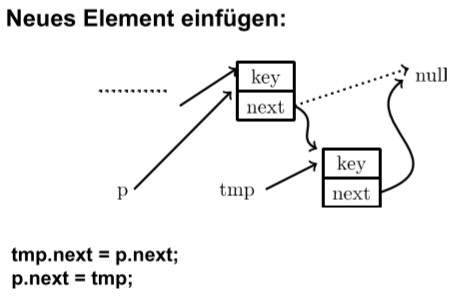
\includegraphics[scale=0.53]{LinkedList_add.jpg}
	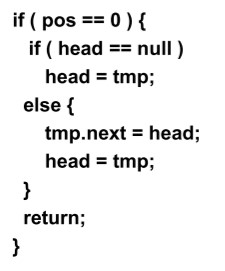
\includegraphics[scale=0.6]{LinkedList_add_code_head.jpg}
	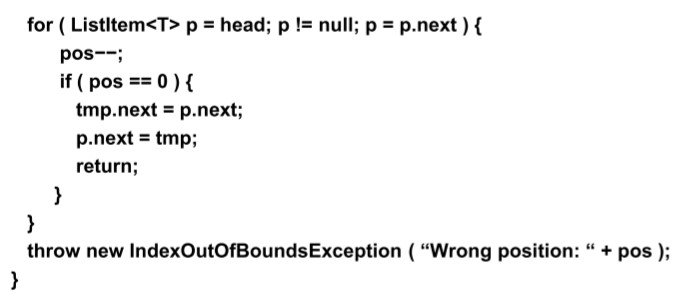
\includegraphics[scale=0.53]{LinkedList_add_code_index.jpg} \\
	$\diamond$
	} 	\\ \hline


	\makecell[l]{Entfernen nach Wert} & 
	\makecell[l]
	{
	$\diamond$ \\
	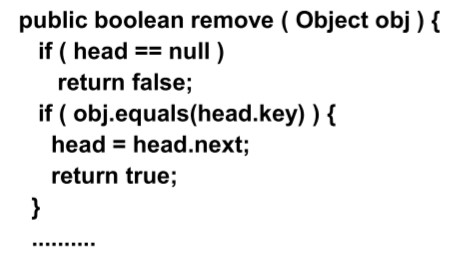
\includegraphics[scale=0.5]{LinkedList_remove_code_head.jpg} \hspace{2cm}
	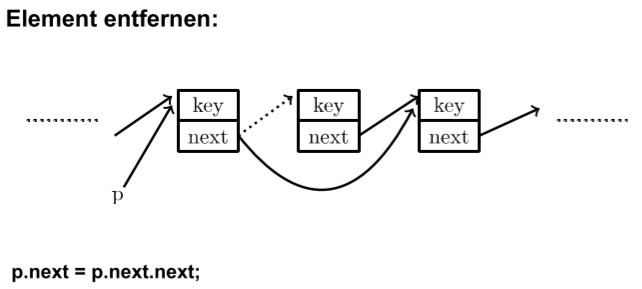
\includegraphics[scale=0.48]{LinkedList_remove.jpg} \\
	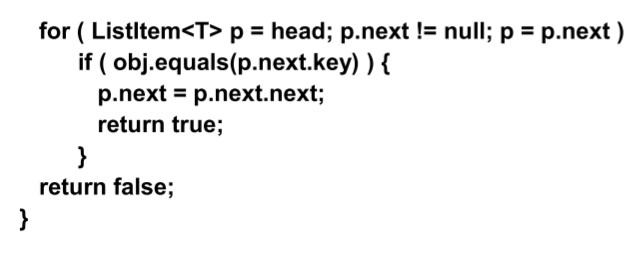
\includegraphics[scale=0.5]{LinkedList_remove_code_object.jpg} \\
	$\diamond$
	} 	\\ \hline


	\end{tabular}
	\end{table}



\section{Optional}


	\begin{table}[H]
	\label{Optional}
	\begin{tabular}{ | p{4cm} p{13.5cm} | }
	

	\hline
	\makecell[l]{Beispiel: Prinziep} & 
	\makecell[l]
	{
	\hspace{0.3cm}  1 \hspace{0.3cm} \texttt{Optional<Number> opt1 = Optional.ofNullable(new Integer(123));} \\
	\hspace{0.3cm}  2 \hspace{0.3cm} \texttt{Optional<Number> opt2 = Optional.ofNullable(null);} \\
	\hspace{0.3cm}  3 \hspace{0.3cm} \texttt{Number n1 = opt1.get();} // n1 == 123\\
	\hspace{0.3cm}  4 \hspace{0.3cm} \texttt{Number n2 = opt2.get();} // NoSuchElementException \\
	\hspace{0.3cm}  5 \hspace{0.3cm} \texttt{Number n3 = opt1.orElseGet(() -> 0);} \\
	\hspace{0.3cm}  6 \hspace{0.3cm} \texttt{Number n4 = opt2.orElseGet(() -> 0);} \\
	} 	\\ \hline


	\makecell[l]{Funktion} & 
	\makecell[l]
	{
	$\rhd$ Aus dem Package java.lang \\
	$\rhd$ Kapselt ein Objekt ein, auch null \\
	$\rhd$ Relativ einfache Methode mit dem Wert null umzugehen \\
	$\rhd$ Die Methode \texttt{orElseGet} entspricht dem Sinn von Optional \\
	$\rhd$ Existiert das Objekt nicht, wird einfach etwas anderes zurückgegeben \\
	$\rhd$ Dies wird durch den Supplier, in dem Fall die Lambda Methode definiert \\
	$\rhd$ Diese gibt bei uns Konstant den int 0 zurück \\
	$\rhd$ Der Rückgabetyp muss von dem selben Typparametern sein wie das Optional \\
	$\rhd$ Optional kann auch ein anderer Lambda Ausdruck benutzt werden \\
	\hspace{0.35cm} für Furnktionen \texttt{ifPresent}, \texttt{map} und \texttt{filter} \\
	} 	\\ \hline


	\makecell[l]{Maps} & 
	\makecell[l]
	{
	as
	} 	\\ \hline


	\end{tabular}
	\end{table}



\section{Streams und Files}


\subsection{Streams}


	\begin{table}[H]
	\label{Streams}
	\begin{tabular}{ | p{4cm} p{13.5cm} | }
	

	\hline
	\makecell[l]{Beispiel: Streams} & 
	\makecell[l]
	{
	\hspace{0.3cm}  1 \hspace{0.3cm} \texttt{List<Number> list = new LinkedList<Number>();} \\
	\hspace{0.3cm}  2 \hspace{0.3cm} \texttt{for(;i<100;) \{ list.add(new Integer(4 + 2*i)) \}} \\
	\hspace{0.3cm}  3 \hspace{0.3cm} \texttt{Stream<Number> stream1 = list.stream();} \\
	\hspace{0.3cm}  4 \hspace{0.3cm} \texttt{Stream<Number> stream2 = stream1.filter(myPred);} \\
	\hspace{0.3cm}  5 \hspace{0.3cm} \texttt{Stream<Number> stream3 = stream2.map(myFuc)} \\
	\hspace{0.3cm}  6 \hspace{0.3cm} \texttt{Optional<Number> opt = stream3.max(new MyNumberComparator);} \\
	} 	\\ \hline


	\makecell[l]{Funktion} & 
	\makecell[l]
	{
	$\rhd$ Generische Klasse Stream
	$\rhd$ Einfache Schnittstelle von Listen, Arrays, Dateien als Sequenz \\
	$\rhd$ \texttt{list.stream()} wandelt eine Liste in einen Stream um \\
	$\rhd$ Genau so kann aus einem Array ein Stream geamcht werden \\
	\hspace{0.5cm} \texttt{Stream<Number> str1 = Arrays.stream(arr);} \\
	$\rhd$ Oder direkt der Inhalt spezifiziert werden \\
	\hspace{0.5cm} \texttt{Stream<Number> str2 = Stream<Number>.of(new Integer(12), ... );} \\
	$\rhd$ Natürlich auch iterieren mit Iterator möglich \\
	} 	\\ \hline


	\makecell[l]{Stream zu...} & 
	\makecell[l]
	{
	$\rhd$ Stream zu List: \\
	\hspace{0.5cm} \texttt{List<String> list = stream.collect(Collectors.toList());} \\
	$\rhd$ Stream zu Array: \\
	\hspace{0.5cm} \texttt{Number[] a = stream.toArray(Number[]::new);} \\
	$\rhd$ Daher heben sich diese Methoden auf: \\
	\hspace{0.5cm} \texttt{Arrays.stream(arr).stream.toArray(Number[]::new)} \\
	} 	\\ \hline


	\makecell[l]{IntStream \\ LongStream \\ DoubleStream} & 
	\makecell[l]
	{
	$\rhd$ Da primitive Datentypen und Generizität nicht kompatibel sind \\
	\hspace{0.35cm} gibt es bei Streams einen Workaround \\
	$\rhd$ So gibt es Streams extra für Primitve Datentypen \\
	} 	\\ \hline


	\makecell[l]{Random Zahlen \\ und Streams} & 
	\makecell[l]
	{
	$\rhd$ So kann man eine Zufällige Zahl erzeugen \\
	\hspace{0.5cm} 1 \hspace{0.4cm} \texttt{Random random = new Random();} \\
	\hspace{0.5cm} 2 \hspace{0.4cm} \texttt{Double x = random.nextDouble();} \\
	$\rhd$ Oder man kann einen Stream von Zufälligen Zahlen erzeugen \\
	\hspace{0.5cm} 1 \hspace{0.4cm} \texttt{IntStream str1 = random.ints();} \\
	} 	\\ \hline


	\makecell[l]{System Streams} & 
	\makecell[l]
	{
	$\rhd$ Die Klasse \texttt{System} besitzt einige Streams: \\
	\hspace{0.4cm} - System.in // Standardmä\ss ig die Tastatur \\
	\hspace{0.4cm} - System.out // Die Konsole \\
	\hspace{0.4cm} - System.err // Fehlerdatie mit allen Errors \\
	$\rhd$ Diese könen gesetzt werden: \\
	\hspace{0.4cm} - System.setIn() \\
	\hspace{0.4cm} - System.setOut() \\
	\hspace{0.4cm} - System.setErr() \\
	} 	\\ \hline

	
	\makecell[l]{Arten von Streams} & 
	\makecell[l]
	{
	$\rhd$ Im Allgemeinen Bauen alle aufeinander auf:
	$\rhd$ BufferedReader(FileReader(Path)) \\
	$\rhd$ PrintStream(BufferedOutputStream(FileOutputStream(Path))) \\
	$\diamond$ \\
	$\rhd$ Für Bytedaten oder ähnliches: \\
	\hspace{0.4cm} - BufferedInputStream \\
	\hspace{0.4cm} - BufferedOutputStream \\
	\hspace{0.4cm} - FileOutputStream \\
	\hspace{0.4cm} - PrintStream \\
	$\rhd$ Für andere Dateien: \\
	\hspace{0.4cm} - Reader // Als Superklasse \\
	\hspace{0.4cm} - FileReader \\
	\hspace{0.4cm} - BufferedReader // Bekommt einen FileReade im Konstruktor \\
	\hspace{0.4cm} - InputStreamReader \\
	\hspace{0.4cm} - BufferedWriter // Bekommt einen FileWriter im Konstruktor \\
	\hspace{0.4cm} - FileWriter \\
	} 	\\ \hline


	\end{tabular}
	\end{table}



\subsection{Files}


	\begin{table}[H]
	\label{Files}
	\begin{tabular}{ | p{4cm} p{13.5cm} | }
	

	\hline
	\makecell[l]{Systemproperties} & 
	\makecell[l]
	{
	$\rhd$ Die Methode \texttt{System.getProperty()} bekommt einen Key \\
	\hspace{0.35cm} und gibt einen String zurück \\
	$\rhd$ Beispiele: \\
	\hspace{0.4cm} \texttt{System.getProperty("user.home")} \\
	\hspace{0.7cm} $\rightarrow$ Gibt den Heimatordner an, bei uns öft der Benutzer Ordner \\
	\hspace{0.4cm} \texttt{System.getProperty("user.dir")} \\
	\hspace{0.7cm} $\rightarrow$ Gibt den Ordner des Programmes an \\
	\hspace{0.4cm} \texttt{System.getProperty("user.name")} \\
	\hspace{0.7cm} $\rightarrow$ Gibt den Benutzer an, der das Programm ausführt \\
	\hspace{0.4cm} \texttt{System.getProperty("file.separator")} \\
	\hspace{0.7cm} $\rightarrow$ Gibt den Systemspezifischen Programmpfad Teiler an \\
	\hspace{1.25cm} Bei Windows oft "$\backslash$", bei UNIX eher "/" \\
	\hspace{0.4cm} \texttt{System.getProperty("line.separator")} \\
	\hspace{0.7cm} $\rightarrow$Gibt den Systemspezifischen Zeilenumbruch an \\
	} 	\\ \hline


	\makecell[l]{Path und Paths} & 
	\makecell[l]
	{
	$\rhd$ Path und Paths dienen dazu Dateipfade zu speichern und zu benutzen \\
	\hspace{0.5cm} 1 \hspace{0.4cm} \texttt{String homeDir = System.getProperty("user.home");} \\
	\hspace{0.5cm} 2 \hspace{0.4cm} \texttt{Path path = Paths.get(homeDir, "fop", "streams.txt");} \\
	$\rhd$ Die Methode get der Klasse Paths bekommt Strings übergeben und \\
	\hspace{0.35cm} setzt daraus einen Dateipfad abhängig vom System, zusammen \\
	\hspace{0.5cm} $\rightarrow$ C:$\backslash$Users$\backslash$Home$\backslash$fop$\backslash$streams.txt \\
	} 	\\ \hline


	\makecell[l]{Lesen von Dateien} & 
	\makecell[l]
	{
	$\rhd$ Es gibt verschiedene Arten Dateien zu lesen \\
	$\rhd$ z.B.: \\
	\hspace{0.5cm} 3 \hspace{0.4cm} \texttt{try (Stream<String> stream = Files.lines(path)) \{} \\
	\hspace{0.5cm} 4 \hspace{0.7cm} \texttt{String fileContent = stream.reduce(String::concat); \}} \\
	$\rhd$ Die Methode reduce erstellt aus allen Teilen eines Streams eine Datei \\
	$\rhd$ Somit kann der Text einer Date eingelesen werden \\
	} 	\\ \hline


	\makecell[l]{Klasse Files \\ Beispiele} & 
	\makecell[l]
	{
	$\rhd$ Dies sind ein paar selbsterklärende Methoden: \\
	\hspace{0.5cm} \texttt{Path paths = Paths.get(...);} \\
	\hspace{0.5cm} \texttt{if (Files.exist(path))} \\
	\hspace{0.5cm} \texttt{if (Files.isReadable(path))} \\
	\hspace{0.5cm} \texttt{if (Files.isWritable(path))} \\
	\hspace{0.5cm} \texttt{if (Files.isRegularFile(path))} \\
	\hspace{0.5cm} \texttt{if (Files.isDirectory(path))} \\
	\hspace{0.5cm} \texttt{long size = File.size(path)} \\
	} 	\\ \hline


	\makecell[l]{Klasse Files \\ Methoden} & 
	\makecell[l]
	{
	$\rhd$ Erstellt eine Datein an dem Pfad: \\
	\hspace{0.5cm} \texttt{Files.createFile(path);} \\
	$\rhd$ Kopiert eine Datei: \\
	\hspace{0.5cm} \texttt{Files.copy(path);} \\
	$\rhd$ Verschiebt oder benennt eine Datei um: \\
	\hspace{0.5cm} \texttt{Files.move(path1, path2);} \\
	$\rhd$ Löscht eine Datei: \\
	\hspace{0.5cm} \texttt{Files.delete(path);} \\
	$\rhd$ Löscht eine Datei, wenn eine vorhanden ist: \\
	\hspace{0.5cm} \texttt{Files.deleteIfExists(path);} \\
	} 	\\ \hline


	\end{tabular}
	\end{table}



\section{Racket: Streams}


	\begin{table}[H]
	\label{Racket Streams}
	\begin{tabular}{ | p{4cm} p{13.5cm} | }
	

	\hline
	\makecell[l]{Funktion} & 
	\makecell[l]
	{
	$\rhd$ Streams in Racket funktionieren änhlich wie in Java \\
	$\rhd$ Leider nicht in DrRacket enthalten \\
	} 	\\ \hline


	\makecell[l]{Beispiel Metehoden} & 
	\makecell[l]
	{
	$\rhd$ Viele Methoden funktionieren wie gwohnt: \\
	\hspace{0.5cm} \texttt{( stream-cons x str )} \\
	\hspace{0.5cm} \texttt{( stream-first str )} \\
	\hspace{0.5cm} \texttt{( stream-rest str )} \\
	\hspace{0.5cm} \texttt{( stream-empty? str )} \\
	\hspace{0.5cm} \texttt{( stream-map fct str )} \\
	\hspace{0.5cm} \texttt{( stream-filter pred str )} \\
	\hspace{0.5cm} \texttt{( stream-fold init fct str )} \\
	} 	\\ \hline


	\end{tabular}
	\end{table}



\section{Exkurs: Methodennamen als Lambda}


	\begin{table}[H]
	\label{Methodennamen als Lambda}
	\begin{tabular}{ | p{4cm} p{13.5cm} | }
	

	\hline
	\makecell[l]{Funktion} & 
	\makecell[l]
	{
	$\rhd$ Etwas omplizierte Angelegenheit \\
	$\rhd$ Kurz gefasst, können Methoden als ersatz für einen Lambda ausdruck stehen \\
	$\rhd$ Oder auch eine Interface Methode ersetzen \\
	$\rhd$ Siehe Scope Identifiert aus C++ \\
	} 	\\ \hline


	\makecell[l]{Beispiel: \\ Gleiche Ausdrücke} & 
	\makecell[l]
	{
	$\diamond$ \\
	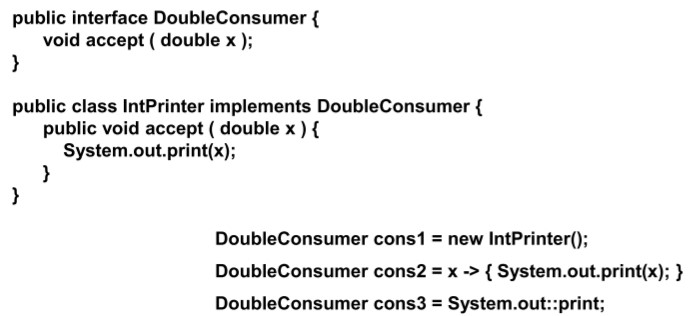
\includegraphics[scale=0.7]{Lambda_ScopeIdentifier_01.jpg} \\
	$\diamond$ \\
	$\rhd$ \texttt{System.out} gibt hier den scope der Methode an \\
	$\rhd$ \texttt{print} ist in dem Fall die Methode \\
	} 	\\ \hline


	\makecell[l]{Erklärung} & 
	\makecell[l]
	{
	$\diamond$ \\
	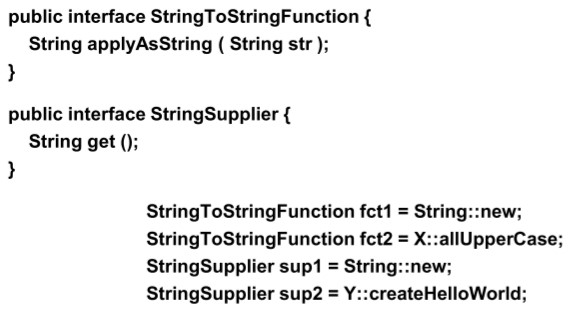
\includegraphics[scale=0.57]{Lambda_ScopeIdentifier_02.jpg}
	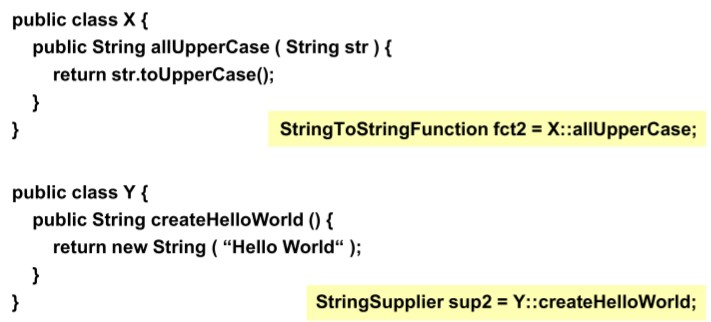
\includegraphics[scale=0.57]{Lambda_ScopeIdentifier_03.jpg} \\
	$\diamond$ \\
	$\rhd$ Der Compiler erkennt, dass die Methode auf die des Interfaces passt \\
	\hspace{0.35cm} und können so Interfaces ersetzt \\
	$\rhd$ So kann auch das Interface \texttt{Function} ersetzt werden \\
	} 	\\ \hline


	\end{tabular}
	\end{table}



\section{Zahlendarstellung}


	\begin{table}[H]
	\label{Zahlendarstellung}
	\begin{tabular}{ | p{4cm} p{13.5cm} | }
	

	\hline
	\makecell[l]{Bitanzahl} & 
	\makecell[l]
	{
	$\rhd$ byte  \hspace{0.5cm}   8 \hspace{0.6cm}  -128 +127 \\
	$\rhd$ short \hspace{0.33cm} 16 \hspace{0.45cm} -32.768 +32.767 \\
	$\rhd$ int   \hspace{0.73cm} 32 \hspace{0.45cm} -2.147.483648 +2.147.483647 \\
	$\rhd$ long  \hspace{0.49cm} 32 \hspace{0.45cm} -9.223.372.036.854.775.808 +9.223.372.036.854.775.807 \\
	} 	\\ \hline


	\makecell[l]{Informationen} & 
	\makecell[l]
	{
	$\rhd$ Die Binär Kodierung einer Zahl nennt man "Bitmuster" \\
	$\rhd$ Jede Ziffer ist asl char ist behält ihre Bitsignatur, \\
	\hspace{0.4cm} zusätzlich werden noch 48 dazu addiert. \\
	$\rhd$ Bei Berechnungen muss dies natürlich wieder abgezogen werden \\
	} 	\\ \hline


	\makecell[l]{2-Komplement} & 
	\makecell[l]
	{
	$\rhd$ Um eine Zahl negativ darzustellen: \\
	$\rhd$ Positive Bitsignatur invertieren, und 1 addieren \\
	$\diamond$ 5: 0101 // negieren \\
	$\diamond$ x: 1010 // und eins addieren \\
	$\diamond$ -5: 1011
	} 	\\ \hline

	\makecell[l]{Gebrochene Zahlen} & 
	\makecell[l]
	{
	$\rhd$ float-Genauigkeit: 1 zu 8.388.608 \\
	$\rhd$ double-Genauigkeit: ca. 1 tz 4,5 Billiarden \\
	$\longrightarrow$ Trotzdem Probleme mit der Genauigkeit \\
	\hspace{0.6cm} Umkehrrechnung liefert möglicherweise nicht das richtige Ergebnis \\
	\hspace{0.6cm} Bei Addition und Subtraktion ungenauigkeit: \\
	\hspace{0.6cm} z.B.: Subtrahieren zweier sehr grö\ss en Zahlen, kann ungenau werden \\
	} 	\\ \hline


	\end{tabular}
	\end{table}



\section{Korrektheit von Software}

\subsection{Korrektheit auf einzelnen Abstraktionsebenen}
	\begin{table}[H]
	\label{Korrektheit auf einzelnen Abstraktionsebenen}
	\begin{tabular}{ | p{4cm} p{13.5cm} | }
	

	\hline
	\makecell[l]{Lexikalische Ebene} & 
	\makecell[l]
	{
	$\rhd$ "Rechtschreibung" - Nicht korrekte Schreibweise von Keywords \\
	$\rhd$ Regeln für Identifier sind festgelegt: \\
	\hspace{0.4cm} \texttt{identifier ::= <<letter>> <<ident-char-list>>} \\
	\hspace{0.4cm} \texttt{ident-char-list ::= $\epsilon$ | <<ident-char>> <<ident-char-list>>} \\
	\hspace{0.4cm} \texttt{ident-char ::= <<letter>> | <<digit>> | \_ | \$ } \\
	\hspace{0.4cm} \texttt{letter ::= a\dots z | A\dots Z} \\
	\hspace{0.4cm} \texttt{digit ::= 0\dots 9} \\
	} 	\\ \hline


	\makecell[l]{Syntaktische Ebene} & 
	\makecell[l]
	{
	$\rhd$ Ähnlich zur Grammatik \\
	$\rhd$ Normalerweise werden diese vom Compiler angefangen \\
	$\rhd$ die Regeln nach denen zu Entscheiden ist ob ein Quelltext \\
	\hspace{0.4cm} ein korrektes Programm in der Sprache ist \\
	\hspace{0.4cm} - Verstö\ss e gegen kontextfreie Regeln \\
	$\rhd$ Typische Fehler enthalten z.B. Klammersetzung: \\
	\hspace{0.4cm} $\diamond$ Zu jeder öffnenden Klammer gehört eine folgende schlie\ss ende Klammer \\
	\hspace{0.4cm} $\diamond$ Niemals überlappende Klammern \\
	$\rhd$ Syntaktische Konstrukte: \\
	\hspace{0.4cm} $\diamond$ Beinhaltet z.B. Köpfe bekannter Schleifen: \\
	\hspace{0.4cm} $\diamond$ \texttt{for (..;..;..)}, \texttt{while (..)}, \texttt{do .. while (..)} \\
	$\rhd$ Auch hier ist eine Formalisierung der Regeln möglich: \\
	\hspace{0.4cm} $\diamond$ \texttt{statement ::= <<compund-statement>> | <<if-statement>> | ...} \\
	\hspace{0.4cm} $\diamond$ \texttt{compund-statement ::= \{ <<statement-sequence>>\} } \\
	\hspace{0.4cm} $\diamond$ \texttt{statement-sequence ::= $\epsilon$ | <<statement>> <<statement-sequence>>} \\
	} 	\\ \hline


	\makecell[l]{Semantische Ebene} & 
	\makecell[l]
	{
	$\rhd$ Werden in der Regel nicht vom Compiler gefunden \\
	$\rhd$ was ein gegebenes Programm tatsächlich macht \\
	$\rhd$ z.B. Runtime Exceptions \\
	$\rhd$ Typische Fehler: \\
	\hspace{0.4cm} $\diamond$ Teilen durch Null \\
	\hspace{0.4cm} $\diamond$ Falsche nutzung des Array Index \\
	\hspace{0.4cm} $\diamond$ Zugriff auf ein nicht exisitierendes Objekt \\
	} 	\\ \hline


	\makecell[l]{Logische Ebene} & 
	\makecell[l]
	{
	$\rhd$ Logische Fehler sind umsetzungs Fehler \\
	$\rhd$ Man weis was das Programm tun soll, setzt es aber nicht richtig um \\
	$\rhd$ Typische Fehler: \\
	\hspace{0.4cm} $\diamond$ off-by-one-error - Mathematische um 1 verrechnet \\
	} 	\\ \hline


	\makecell[l]{Spezifikatorische Ebene} & 
	\makecell[l]
	{
	$\rhd$ Bereits der umzusetzende Gedanke war Falsch \\
	$\rhd$ Beispiel 2000-Fehler: \\
	\hspace{0.4cm} $\diamond$ Nicht erwartet, dass Programma bis und nach 2000 im Betrieb sind \\
	\hspace{0.4cm} $\diamond$ Daher Jahreszaahl codierung nur mit 2 Ziffer statt 4 \\
	} 	\\ \hline


	\end{tabular}
	\end{table}



\subsection{Korrektheit von Software}
	\begin{table}[H]
	\label{Korrektheit von Software}
	\begin{tabular}{ | p{4cm} p{13.5cm} | }
	

	\hline
	\makecell[l]{Überblick} & 
	\makecell[l]
	{
	$\rhd$ Kein Programmabbruch durch Fehler \\
	$\rhd$ Termination \\
	\hspace{0.4cm} $\diamond$ wenn Aufgabe erledigt oder \\
	\hspace{0.4cm} $\diamond$ wenn Befehl zur Termination von au\ss en \\
	$\rhd$ Korrekte Ausgaben und Effekte \\
	} 	\\ \hline


	\makecell[l]{Korrektheit von Klasse} & 
	\makecell[l]
	{
	$\rhd$ Darstellungsinvariante (representation invariant) von Klassen u. Interfaces \\
	\hspace{0.4cm} $\diamond$ Beschreibt Darstellung der Objekte gegenüber Nutzer und Klasse \\
	\hspace{0.4cm} $\diamond$ Die Sicht, die Attribute und Methoden vermitteln, die public sind \\
	$\rhd$ Implementationsinvariante (implementation invariant) von Klassen \\
	\hspace{0.4cm} $\diamond$ Analog zur Darstellungsinvariante \\
	\hspace{0.4cm} $\diamond$ Behandelt den Teil der Klassendefinition, der nicht public ist \\
	$\rhd$ Liskov Substitution Principle (LSP): \\
	\hspace{0.4cm} $\diamond$ Jede Aussage über das logische Verhalten der Basisklasse, \\
	\hspace{0.8cm} muss auch für die abgeleitete Klasse gelten. \\
	$\rhd$ Zusammenfassend: \\
	\hspace{0.4cm} $\diamond$ Die Darstellungsinvariante und, soweit es die protected Attribute betrifft, \\
	\hspace{0.8cm} auch die Implementationsinvariante müssen immer eingehalten werden \\
	} 	\\ \hline


	\makecell[l]{Korrekthiet von \\ Subroutinen} & 
	\makecell[l]
	{
	$\rhd$ Subroutine als Oberbegriffe für Methoden und Funktionen \\
	$\rhd$ Zweiter Teil des LSP: \\
	\hspace{0.4cm} $\diamond$ Vorbedingung darf nur abgeschwächt, nicht verschärft oder ersetzt \\
	\hspace{0.4cm} $\diamond$ Nachbedingung darf nur verschärft, nicht abgeschwächt oder ersetzt \\
	} 	\\ \hline


	\makecell[l]{Korrektheit von \\ rekursiven Subroutinen} & 
	\makecell[l]
	{
	$\rhd$ Rekursionsabbruch \\
	\hspace{0.4cm} $\diamond$ Muss vorhanden sein, damit Rekursion ordentlich terminiert \\
	$\rhd$ Rekursionsschritt \\
	\hspace{0.4cm} $\diamond$ Schritt näher an den Rekursionsabbruch \\
	$\rhd$ Beweies der Korrektheit mittels Induktion \\
	\hspace{0.4cm} $\diamond$ Induktionsbehauptung: Aufstellung für Problemgrö\ss e \\
	\hspace{0.4cm} $\diamond$ Induktionsanfang: z.B. Problemgrö\ss e = 1 \\
	\hspace{0.4cm} $\diamond$ Induktionsvorraussetzung: Der Vertrag gelte für ... \\
	\hspace{0.4cm} $\diamond$ Induktionsschritt: z.B. Verringerung der Listenlänge \\
	} 	\\ \hline


	\makecell[l]{Korrektheit in \\ Subroutine: Schleifen} & 
	\makecell[l]
	{
	$\rhd$ Schleifeninvariante: Aussagen darüber, was sich während Schleife nicht ändert \\
	\hspace{0.4cm} $\diamond$ Formulierung "Nach h $\geq$ 0 Schritten ist ..." \\
	\hspace{0.4cm} $\diamond$ Verwendung einer Variable $h$ die nicht im Code vorkommt \\
	$\rhd$ Schleifenvariante: Aussagen darüber, was sich während der Schleife ändert \\
	\hspace{0.4cm} $\diamond$ Formulierung: for: "h steigt um 1" $\rightarrow$ Zusammenfassung: \\
	\hspace{0.4cm} $\diamond$ Formulierung: "Nach Schleifenende ..." \\
	$\rhd$ Indukion bei Schleifen: \\
	\hspace{0.4cm} $\diamond$ Invariante = Induktionsbehauptung: "Nach h $\geq$ 0 Schleifendurchläufen gilt.." \\
	\hspace{0.4cm} $\diamond$ Induktionsanfang, also h=0: "Die Initialisierung vor der Schleife sorgt dafür, \\
	\hspace{0.75cm} dass die Invariante unmittelbar vor dem ersten Druchlauf erfüllt ist." \\
	\hspace{0.4cm} $\diamond$ Induktionsvorraussetzung für h>0: "Die Invariante gelte für h-1." \\
	\hspace{0.4cm} $\diamond$ Induktionsschritt: "Unter Voraussetzung, dass..., nach h Druchläufen gilt." \\
	} 	\\ \hline


	\end{tabular}
	\end{table}



\section{Effizienz von Software}

\subsection{Nebenaspekte der Effizienz}
		\begin{table}[H]
		\label{Nebenaspekte der Effizienz}
		\begin{tabular}{ | p{4cm} p{13.5cm} | }
		
	
		\hline
		\makecell[l]{Lexikalische Ebene} & 
		\makecell[l]
		{
		$\rhd$ "Rec
		} 	\\ \hline
	
	
		\makecell[l]{Syntaktische Ebene} & 
		\makecell[l]
		{
		$\rhd$ Ähnlich 
		} 	\\ \hline
	
	
		\makecell[l]{Semantische Ebene} & 
		\makecell[l]
		{
		$\rhd$ Werden
		} 	\\ \hline
	
	
		\makecell[l]{Logische Ebene} & 
		\makecell[l]
		{
		$\rhd$ Logische
		} 	\\ \hline
	
	
		\makecell[l]{Spezifikatorische Ebene} & 
		\makecell[l]
		{
		$\rhd$ Bereits der um
		} 	\\ \hline
	
	
		\end{tabular}
		\end{table}



\subsection{Hauptaspekte der Effizienz}
		\begin{table}[H]
		\label{Hauptaspekte der Effizienz}
		\begin{tabular}{ | p{4cm} p{13.5cm} | }
		
	
		\hline
		\makecell[l]{Lexikalische Ebene} & 
		\makecell[l]
		{
		$\rhd$ "Rec
		} 	\\ \hline
	
	
		\makecell[l]{Syntaktische Ebene} & 
		\makecell[l]
		{
		$\rhd$ Ähnlich 
		} 	\\ \hline
	
	
		\makecell[l]{Semantische Ebene} & 
		\makecell[l]
		{
		$\rhd$ Werden
		} 	\\ \hline
	
	
		\makecell[l]{Logische Ebene} & 
		\makecell[l]
		{
		$\rhd$ Logische
		} 	\\ \hline
	
	
		\makecell[l]{Spezifikatorische Ebene} & 
		\makecell[l]
		{
		$\rhd$ Bereits der um
		} 	\\ \hline
	
	
		\end{tabular}
		\end{table}





\end{document}